%!TEX root = ../thesis.tex

\chapter{Methodology and methods}
\label{chap:mm}

This first section of this chapter presents a description of the methodology of the planned dissertation work. This description is limited to matters relating to planning the execution of the work, without going into specifics about the methods themselves. The second section of the chapter presents an overview of the methods themselves, including information about how these plans evolved since the P2. This section also includes detailed accounts of the thought processes leading to the most important design choices. The rest of the chapter is devoted to a detailed account of the methods that underlie each of the processing steps in the final "proof-of-concept" software implementation, with accompanying flowcharts to illustrate the system design represented by the methods. A short section at the end of the chapter describes the implementation's software architecture, with explanation about certain technical design choices regarding the implementation.

\section{Methodological framework}
\label{sec:methodology}

This section contains a written account of the key stages into which the execution of this research can be divided. Each subsection describes one such stage, discussing the specific tasks performed during each stage as well as what has changed relative to my original plans. The methodology is also visually illustrated on a flowchart in Figure \ref{fig:methodologyflow}.

\subsection{Preparation}
\label{sub:preparation}

This project concerns a client - NDW - with specific requirements and a pre-existing attempt at implementing a solution, in addition to aspects that are purely scientific. As a result, the first stage of the project involved \textit{consultation with the client} and with their commercial developers - RHDHV - in addition to the task of \textit{familiarising myself with the research topic and literature}. The results of these preparation tasks were \textit{discussed internally} with my supervisors and used to \textit{define the final list of formal research questions} on the basis of focusing primarily on academic topics while also fulfilling the requirements of the client. This combined knowledge was then used to \textit{produce the P1 submission}. This stage roughly coincided with Q1 of the academic year, and with the P1 period of the dissertation research.

I executed this stage of the project according to my initial plans, little has changed during its realisation.

\subsection{Preliminary analysis, proposal writing}
\label{sub:preliminaryanalysis}

The second stage of the project involved \textit{further consultation with the client and their developers} to determine to what extent the commercial and scientific branches of the 3D-NDW project could be linked, and to allow me to understand the exact methods used in the prototype and the commercial implementation (which was being actively developed during this period of time). In parallel with these tasks, I \textit{performed the necessary in-depth literature review} and preliminary analysis. The preliminary analysis was comprised  of a \textit{close examination of the input datasets and their documentations} (input assessment), and based on this and the research questions, the \textit{final selection of relevant concepts and methods}. I also selected a range of illustrative geographical regions during the preliminary analysis, and cropped the datasets to their extents to \textit{create testing input files} for later development and testing. Lastly, the results of this stage were distilled to \textit{produce the P2 document}. This stage roughly coincided with Q2 of the academic year, and with the P2 period of the dissertation research.

I executed this stage of the project according to my initial plans, but with a few small alterations. My initial plan was to put a slightly larger emphasis on performing preliminary analysis tasks, but the abundance of relevant literature and the complex task of creating a preliminary design for the methods (and the pipeline itself) limited the amount of time I could spend on it. I focused most of my effort at this stage in the research on the litrature review and the preliminary system design instead. This meant that during the next stage, I had a solid starting point in terms of background knowledge, and specific plans regarding what to start implementing.

\subsection{Analysis}
\label{sub:analysis}

The third stage of the research spanned the period between my P2 and P4 presentations. This stage concerned carrying out most of the analysis. The period was characterised first and foremost by the intense development effort focused on the \textit{implementation of individual algorithms and steps of the workflow}. My original plan was to isolate this set of tasks and perform it during the period between my P2 and P3 presentations, and to \textit{assemble the pipeline} from the individual modules after the P3. However, it proved to be more effective to develop the modules and incrementally extend the pipeline with them at the same time - an approach to which I switched after implementing the first few modules. This allowed me to resolve pipeline-level issues as part of the incremental refinement of methods, in addition to problems related to specific pipeline steps only.

Carrying out the \textit{accuracy-related analysis} was the last stage of the project that required active development on the program code. Testing the individual procedures and the pipeline was continuous during the implementation, with larger tests performed after reaching major milestones. Testing, and the assessment of performance and accuracy used the testing datasets I produced as part of the preliminary analysis. This was followed by a self-evaluation of the overall results of the research and a discussion of them with my supervisors, as well as a comparison of the commercial results and mines. The stage was concluded by \textit{writing the present draft thesis} ahead of my P4 presentation.

\subsection{Finalisation}
\label{sub:finalisation}

The last stage of the project will last a few weeks between the P4 presentation and the P5 presentation. Both \textit{the implementations and the present report itself will be improved and finalised} during this time. The final version of the source code and its documentation will be published in the project repository on GitHub. Furthermore, the outcome of the research and its findings relevant to improving the commercial implementation will be discussed with our client.

\begin{figure}
    \centering
    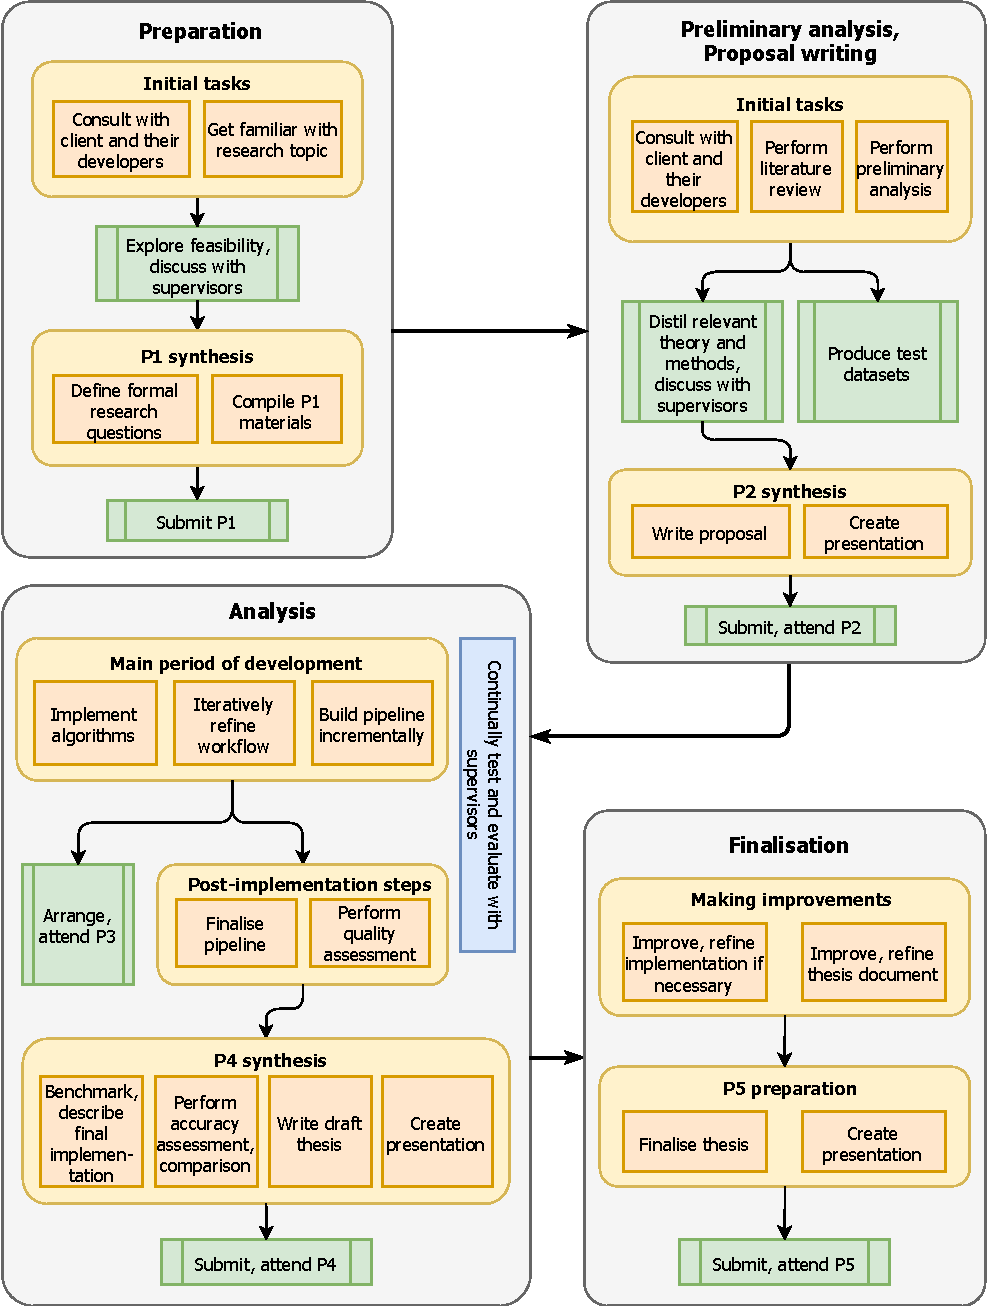
\includegraphics[width=0.9\linewidth]{final_report/figs/methodology.pdf}
    \caption{Flowchart-style illustration of the top-level methodology of my dissertation research.}
    \label{fig:methodologyflow}
\end{figure}

\section{Overview of methods}
\label{sec:methodsoverview}

This section provides a structured overview of the steps of the processing pipeline. While the detailed descriptions in Section \ref{sec:methods} focus on explaining how exactly each step works, the purpose of the present section is to provide the rationale justifying their necessity and the reasons underlying certain major design choices, as well as to describe their role in the context of the system as a whole.

While the exact aims of the project materialised during the first two stages listed in Section \ref{sec:methodology} above, a brief description of the project existed before it. The project was originally conceived as a an academic continuation to the pre-existing attempt of NDW to implement a solution to the 3D conversion of NWB, re-using NDW's prototype implementation as the basis for a completed, academically sound version. During the aforementioned two stages, it became clear that NDW's pre-existing implementation is not robust and flexible enough to justify building the academic project on top of it. Hence, the entirety of the below pipeline was designed and implemented specifically for this academic project, no part of it represents code borrowed from the NWD prototype (or the RHDVH implementation).

\subsection{Proposed processing pipeline}
\label{sub:pipelineoverview}

The design of the pipeline is the result of a combined understanding of concepts described in related work, my own knowledge and experience relating to the geomatics discipline, as well as inspiration from the methods of the commercial implementation. The proposed workflow was built with a strong focus on finding answers to the research questions. Furthermore, it is also the result of a process of iterative refinement. In most cases, this only concerns the technical details of the algorithms implementing the pipeline steps, but in some cases I also made major changes to certain aspects of the general approach. Hence, in the structured overview below, I added a list item per pipeline step specifically to describe what changes, if any, were made to the given step.

As a brief summary of the general idea, the pipeline takes NWB, decomposes it into roads whose surface can be modelled by 2.5D methods, and applies a set of mostly geomatics operations to produce the 2.5D road surface models that the elevations are then derived from to produce 3D-NWB. Accuracy-related considerations are not yet described in this section, these are first discussed in Section \ref{sub:accuracyoverview} below. A visual illustration of the main pipeline steps is shown in Figure \ref{fig:workflow}, showing only the titles of each workflow step in the order in which they are executed.

\begin{figure}
    \centering
    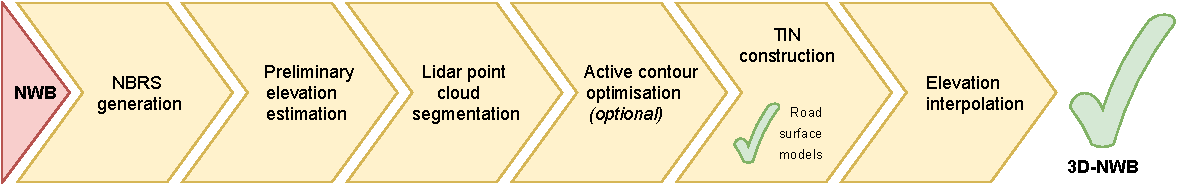
\includegraphics[width=0.9\linewidth]{final_report/figs/workflow_steps.pdf}
    \caption{Illustration of the top-level steps and output of my processing pipeline.}
    \label{fig:workflow}
\end{figure}

\begin{enumerate}
    \item \textbf{NBRS generation}
    \begin{enumerate}
        \item \textbf{Goal:} assemble optimal 2D profiles from the building blocks of NWB.
        \item \textbf{Approach:}
        \begin{enumerate}
            \item Assemble \textit{Non-Branching Road Segments}, henceforth referred to as \textit{NBRS} (in both plural and singular) from NWB geometry. To do so, look for series of NWB wegvakken (LineString objects) that represent the same road and join them into optimised 2D profiles - NBRS.
            \item Perform the assembly of NBRS in a way that maximises their length (optimal for lengthwise 2D operations such as polynomial fitting), minimising internal angles at the same time. Disallow self-intersection, so that each NBRS can be modelled in 2.5D.
        \end{enumerate}
        \item \textbf{Purpose:} this step is necessary, because in addition to working with small-scale (short wavelength) features in the road network, we wish to be able to inspect trends that take place over longer distances in the network. The building blocks of NWB (wegvakken) can sometimes be short, occasionally only a few metres long. Hence, assembling them into NBRS provides a better starting point for later steps.
        \item \textbf{Changes:} from the outset, I expected that simple methods based on progressing along 2D profiles, as well as modelling 2D profiles as a whole, would be useful for this project, and that a data structure serving this dual purpose would be necessary. Hence, NBRS have always been part of my plans and their exact specifications did not change much during development.
    \end{enumerate}
    \item \textbf{Preliminary elevation estimation}
    \begin{enumerate}
        \item \textbf{Goal:} create a rough, preliminary 3D version of NWB.
        \item \textbf{Approach:}
        \begin{enumerate}
            \item Based on the median elevation of nearby Lidar points, associate NBRS vertices with preliminary elevation approximates, thereby performing a crude 3D conversion of NWB.
            \item Perform polynomial fitting on the 2D profiles that NBRS represent. Identify vertices that are outliers with respect to the general shape of the NBRS and interpolate values for them linearly.
        \end{enumerate}
        \item \textbf{Purpose:} this step is necessitated by the next one, point cloud segmentation. While it is possible to perform it without first performing a rough 3D conversion, I found it to be much more effective when the approximate 3D locations of NBRS are already known by that point.
        \item \textbf{Changes:} this step represents and addition relative to the original plans. I started suspecting its benefits during the implementation stage, and subsequently added it to the pipeline design.
    \end{enumerate}
    \item \textbf{Point cloud segmentation}
    \begin{enumerate}
        \item \textbf{Goal:} using their preliminary elevations, find "patches" of Lidar points in the 3D vicinity of NBRS vertices. Progressing along the vertices of each NBRS in a linear manner, fit planes on their Lidar patches. Where an unexpected change in the plane fits is detected, rely on DTB to provide a reference and to help navigate through the ambiguous region.
        \item \textbf{Approach:}
        \begin{enumerate}
            \item Where DTB is also unavailable, accept the shifted (or missing) plane fits but perform a polynomial fit afterwards to identify planes that are unlikely to belong to the relevant road surface. Split the NBRS into parts in such places, excluding the undesired regions from further consideration until the last pipeline step. 
            \item Based on the plane fits, decide which points in the patches are relevant to the road surface represented by a given NBRS, and create subclouds by merging them (one for each NBRS part). Include DTB points that were used in places where AHN3 data was missing.
        \end{enumerate}
        \item \textbf{Purpose:} like NBRS generation, this step also has a dual purpose. Firstly, it associates each NBRS with a set of candidate Lidar and DTB points that are likely to be relevant to them, thereby reducing the amount of Lidar points that will need to be processed later on. Secondly, it also excludes the majority of points which are close to a given road, but which were reflected from occluding geometry instead of its surface.
        \item \textbf{Changes:} originally, I only wished to detect where plane fits become inconsistent to exclude small-scale occlusion at this point. However, I eventually realised that by tracking changes in certain metrics, I could do so even in relatively long occluded regions. I then incorporated DTB as a backup dataset to increase the reliability of this method, which made the solution work even where significant changes in elevation take place inside the occluded regions (such as in tunnels). I added the splitting of NBRS into parts as a last tweak, after implementing the rest of the pipeline. This improved the results of later steps by removing areas without AHN3 \textit{and} DTB coverage from the NBRS.
    \end{enumerate}
    \item \textbf{Preliminary edge approximation}
    \begin{enumerate}
        \item \textbf{Goal:} create line geometries on both sides of NBRS approximating the edges of the road surfaces.
        \item \textbf{Approach:}
        \begin{enumerate}
            \item construct cross-sections on NBRS vertices and convert them to 2D elevation profiles by sampling AHN3 along their length. Perform linear regression on each, and select the outermost stable inlier points on both sides of the NBRS. The two points are taken to represent the road edge locally.
            \item Assemble approximate road edges from the discrete edge points generated by the previous step, enforcing constraints regarding the expected shape of the road edges. Relax the constraints after a certain number of successive failures, to allow the algorithm to adapt to real-life changes in the road geometry.
        \end{enumerate}
        \item \textbf{Purpose:} the sole purpose of this step was going to be to provide edge estimates for active contour optimisation. After I made the decision to make active contour optimisation optional in the pipeline (due to its ineffectiveness), preliminary edges also became optionally needed for later steps, in place of the optimised contours.
        \item \textbf{Changes:} Due to the optional use of preliminary edges in TIN construction (in case optimisation is skipped), I needed to improve their quality significantly. This entailed the implementation of significant refinements to the underlying algorithm, as well as the constraints enforcement steps that I mentioned above.
    \end{enumerate}
    \item \textbf{Active contour optimisation \textit{(optional)}}
    \begin{enumerate}
        \item \textbf{Goal:} refine the preliminary edges based on road surface smoothness as described by Lidar.
        \item \textbf{Approach:}
        \begin{enumerate}
            \item Construct an attractor map from the subcloud of each NBRS part, based on a scalar metric describing the local smoothness of the points.
            \item Use the preliminary edges and the attractor maps to perform active contour optimisation.
            \item Find a parametrisation for the active contour optimisation algorithm that works well with all testing datasets.
        \end{enumerate}
        \item \textbf{Purpose:} the original purpose of this step was to optimise the preliminary edges to the extent where they can be used to classify subcloud points either as surface or non-surface points. Since this was found not to work reliably, the current purpose of the step could be described as \textit{simplifying and enhancing the shapes of the preliminary edges}.
        \item \textbf{Changes:} even after improving all prior steps of the pipeline and sufficiently refining the parametrisation, the algorithm still produces mediocre results. As a result, I eventually implemented a bypass so that it can be skipped. Furthermore, I originally planned to apply morphological operations to attractor maps composited from maps generated using multiple different metrics. I found this to be ineffective in practice, the final implementation simply uses the raw results of the sole best-performing metric.
    \end{enumerate}
    \item \textbf{TIN construction}
    \begin{enumerate}
        \item \textbf{Goal:} model each NBRS part by a TIN based on the subclouds and preliminary or optimised edges.
        \item \textbf{Approach:}
        \begin{enumerate}
            \item Seed each TIN by inserting points around the centre of the road unconditionally. Define the "centre of the road" based on the \textit{edges}, not the 2D location of the underlying NWB centreline of the NBRS part.
            \item Initialise each TIN by conditionally inserting points within the preliminary or optimised edges.
            \item Extend each TIN by conditionally inserting points further and further away from the centre of the road, beyond the edges if desired. 
        \end{enumerate}
        \item \textbf{Purpose:} this step also serves a dual purpose. On one hand, it satisfies our academic interest in creating 2.5D surface models of the roads. On the other hand, these models can then be used to interpolate final elevations for NWB efficiently. Lastly, as the TIN consists of input elevation measurements, it allows output accuracy to be estimated in a straightforward manner.
        \item \textbf{Changes:} the original idea for this step was that the optimised road edges would be hard-coded in the TIN (a CDT was planned), and only points within these constraint geometries would be inserted. Due to the ineffectiveness of active contour optimisation, I instead needed to create a TIN construction workflow that can make the best of the edges and subclouds \textit{without} making the assumption that the edges have near-perfect accuracy.
    \end{enumerate}
    \item \textbf{Elevation interpolation}
    \begin{enumerate}
        \item \textbf{Goal:} derive a final elevation for each NWB vertex while enforcing continuity across intersections, and augment the original dataset with the results.
        \item \textbf{Approach:}
        \begin{enumerate}
            \item Interpolate in the respective TINs to obtain a final elevation value for each vertex of each NBRS part.
            \item At intersections, use the first elevation that was interpolated at that approximate 3D location and connect (snap) all other NBRS to it that end or begin at that intersection.
            \item Use linear interpolation to fill in elevations in NBRS where TIN-based interpolation was not possible.
            \item Mark the origin of each output elevation either as AHN3, DTB or linear interpolation.
        \end{enumerate}
        \item \textbf{Purpose:} obtain the final NWB elevations and output 3D-NWB, keeping a record of which elevation comes from where.
        \item \textbf{Changes:} originally, I thought that enforcing continuity across intersections was going to be a bigger challenge. However, I found the TIN representations of the same intersections across different NBRS to be consistent reliably, hence interpolating a single elevation (based on the first NBRS part encountered) and snapping all subsequent ones to it works without issues in almost all scenarios examined.
    \end{enumerate}
\end{enumerate}

I was inspired by concepts and ideas from related work (see Chapter \ref{chap:rw}) while designing the original pipeline, and the final implementation retains many of these similarities. For instance, the point cloud segmentation step was inspired largely by \cite{oudeElberink_vosselman_2009} and \cite{boyko_funkhauser_2011}. The cross-section based edge detection workflow was inspired by curb detection-related work, such as \cite{yang_etal_2013} and the methods of the commercial implementation. The use of 2.5D-based modelling methods to represent surfaces extracted from the point cloud comes from \cite{oudeElberink_vosselman_2006}. The active contour-based workflow was inspired by \cite{boyko_funkhauser_2011} and \cite{gopfert_etal_2011}. In a way, my work can also be interpreted as a study of the effectiveness of relevant methods commonly found in the literature.

\subsection{Dependency of methods on specific datasets}
\label{sub:m_generalisation}

In this report I commonly refer to DTB as a \textit{support dataset}. This is in part due to it always having been secondary to AHN3 because its spatial coverage is vastly inferior to AHN3 and it could not, by itself, fulfil the role AHN3 was given in this project, whch may therefore be called the \textit{primary dataset}. AHN3 contains enough data to make it possible to run the pipeline in the complete absence of DTB. DTB merely improves the results of the point segmentation step and extends the TINs into areas not covered by AHN3 (preventing them from being split into parts in the process).

The reason why I often refer to the two elevation sources in such as way, is that it describes their \textit{roles} rather than their exact \textit{identity}. For the same reason, I also often refer to NWB simply as the "road network". This is in line with my goal to make my methods as independent from the exact identity and properties of AHN3, DTB and NWB as possible. Most parts of my methods should work regardless of the exact datasets used, as long as a few assumptions are satisfied. For instance, the primary Lidar dataset needs to be accurately classified, in particular vegetation should be clearly isolated from ground reflections. DTB could also be replaced with any generic dataset that contains accurate 3D geometries representing the surfaces of the relevant roads - or better still, with MLS data providing coverage where the primary ALS one does not. The main difference is in scale between the primary and the support dataset; the purpose of the latter is to introduce data where the primary dataset has data \textit{gaps}.

The main concerns regarding generalisation (how well the methods and the implementation work independently from the properties of the datasets) are not related to the input datasets, but to the parametrisation of certain parts of the implementation. While many such parameters are exposed as arguments and can be customised by the user, there are also many that are hard-coded to avoid creating an API with an inconveniently long list of arguments. While the default parametrisation works in all the study areas of this project, there is no guarantee that they would always work equally well with other datasets - especially with ones containing road networks that possess different properties than that of The Netherlands (e.g. mountainous areas). However, being an open-source, proof-of-concept software, there is nothing to prevent potential reusers of my code from adapting it to their needs, including making changes to its fixed parametrisation.

\subsection{A note on DTB's role}
\label{sub:generalisation}

In my P2 document, no specific mention was made about the role intended for DTB, but a section was dedicated to speculating about potential uses. The evolution of its role in the final implementation was entirely up to the iterative refinement of the methods. In the end, the deciding factor in determining how DTB could be used was that I found it to be useful for patching in gaps in AHN3 coverage, which is how the roles of primary and secondary dataset for AHN3 and DTB came about.

Among potential uses I speculated about before starting the development was the use of DTB as a means of contributing to edge estimation/optimisation, and to the lateral refinement of NWB positions. However, I found DTB road markings to be missing most commonly in the exact locations where they could have contributed to these aspects, for instance in sharp bends.

Using DTB as a secondary dataset with the sole intention of characterising occluded road surfaces also generalises better, as the previous section makes clear. Consultations with NDW also made it clear that they are in the position to commission the survey of additional georeferenced points or lines from Kragten (via a vehicle on which which commercial GNSS systems are mounted) or to purchase MLS data from Cyclomedia. Unlike DTB, such data would \textit{not} correspond to specific road markings.

These circumstances are what prompted me to treat DTB in a more generic manner, and to then extend this mindset to the way the rest of the datasets are used in my methods.

\subsection{Accuracy assessment of processing steps}
\label{sub:accuracyoverview}

As I emphasised in various places in this report already, it was among the aims of this research to perform the 3D conversion of NWB in a way that output accuracy is as close the the input accuracy as possible, and that it can be evidenced and quantified either for the process as a whole, or for each output vertex individually.

As the literature review results in Chapter \ref{chap:rw} already indicated, there are various ways to go about this problem. The first and foremost decision one needs to make is whether an empirical or a theoretical approach is better suited to the given procedure. For our procedure, both appeared equally suitable at first. I first attempted an empirical approach, but having produced uncharacteristic results using this approach, I eventually settled on a combination of simple decision-making logic and a theoretical, mathematical framework. I will provide the details about the procedures later in this chapter, in Section \ref{sec:m_accuracyassessment}.

Below, I will outline the general approach, and the assumptions that are made when using it.

\subsubsection{Assumptions about influences}

My system design interpolates the output elevations from a TIN whose vertices are the Lidar road surface measurements themselves. I opted for this approach specifically because my literature review indicated that interpolating in such a DTM appears to be the best option for large-scale terrain as well as in terms of accuracy, and because - assuming perfect ground filtering - it introduces no errors relative to the original Lidar data. However, as I explained in Section \ref{sec:lidaraccuracy}, the output accuracy in such a process is a factor of not only the generated DTM and the interpolation technique used, but also of local, "environmental" factors. I made a range of assumptions regarding these influences before proceeding to the accuracy estimation step, which I will explain below.

The first factor to consider is the local \textit{accuracy of ground filtering}. In this project, most of the Lidar data was already ground filtered, as I made use of the excellent stock classifications that are present in AHN3 (please refer to Section \ref{sub:ahn} for more information on this topic). There is one exception to this rule: roads found on bridges were manually classified as bridges, including all objects on the roads such as guardrails and vehicles. Using the bridge classification also added objects over other roads (such as motorway signs), which locally violate the assumption that the road surfaces are ground-filtered.

However, processing steps in this research remove most non-road reflections from above road surfaces, and any remaining ones are eliminated by the careful conditional insertions of the TIN construction step. This holds both in theory and practice, as \ref{chap:r} explains. The number of outliers \textit{on road surfaces} is so small, that if we make the assumption that we only wish to interpolate elevations on road surfaces, we may regard the theoretical ground filtering effectiveness to be 100\%. As a result, the influence of non-road reflections (outliers on road surfaces) needs not be considered in the accuracy assessment.

The second factor to consider is the local sampling density of the Lidar points (and DTB, where it was used in place of AHN3). The assumption I made here is that as long as the TIN locally conforms with the theoretical minimum Lidar sampling density required to characterise a flat surface without oversampling it, the output accuracy will be not suffer from any detrimental influence. I implemented simple logics to detect where interpolation has taken place in a location where the sampling density drops below this level. Vertices interpolated in such triangles do not receive an output accuracy value, and are thus flagged as having \textit{undetermined} accuracy. The details regarding the identification of a suitable local density threshold is found in Section \ref{sub:m_accuracypoorsampling} later in this chapter.

This second assumption holds, because in flat areas that are \textit{oversampled} by Lidar, literature indicates sampling density to have little to no correlation with empirically-derived error. In such areas, oversampling already occurs at point densities far lower than what is typical of AHN3, apart from places where there are gaps in the data. Hence, a simple threshold-based evaluation can be deemed a sufficient measure to deal with the influence of this factor. This decision was made in view of the results of my empirical accuracy assessment results, which also indicated no correlation between sampling density and TIN model accuracy (see Section \ref{sub:accuracyempirical} for the details).

The last non-interpolation influence to consider is that, which is caused by terrain slope and ruggedness. Relevant literature discussed this topic also in the context of local sampling density, because it is especially in sparsely-sampled regions small, local variations that the ruggedness introduces may not be captured adequately. Road surfaces are, however, smooth. Furthermore, even inclined roads in our datasets are always characterised by smooth, gradual slope transitions - which makes sense, considering that both the motorways and municipal roads we are working with have high speed limits. The effects of local curvature on accuracy in this case may be neglected.

This combination of factors and assumptions lead me to implement an accuracy assessment workflow that either deems the accuracy to be undetermined (where sampling density is very low) or computes its accuracy solely based on the principles of error propagation through TIN-linear interpolation. This error propagation method predicts an \textit{increase} in the the standard error relative to that of the input for surfaces that are not very steeply inclined. The two categories also correspond with whether the output conforms with the requirements of the noise regulations or not. The details of this are found in \ref{sub:accuracyformal}.

\subsubsection{Influence of other steps}

It may strike the reader as odd that it is almost only the last two pipeline steps that are discussed above in terms of what defines output accuracy. The reason behind this is that the TINs are constructed entirely of AHN3 and DTB points, thus making the standard vertical and horizontal error of each TIN node known. If the TINs were constructed from points which were themselves "secondary information" (i.e. derived information) relative to the input, then the estimation of output accuracy would be more involved. However, this is not the case here - and therefore, wherever the above three assumptions hold, the quality of the TIN and the interpolation technique define the output accuracy alone.

The rest of the pipeline steps only affect whether the above assumptions are violated in a certain place or not. In particular, they may affect the local density of vertices in the TINs and whether a TIN exists at the 2D location of a particular NWB vertex or not. If we focus only on the influence of processing steps (i.e. we ignore the effects of physical factors and problems with the data), this may for instance be the result of a very poor polynomial fit in the preliminary elevation estimation step causing Lidar segmentation to fail locally, or the rare cases where preliminary edge estimation fails too many times in a row. Such blunders may cause issues in the TIN, but these too, will be picked up by the threshold-based evaluation and classified as unreliable accordingly.

Furthermore, we must also consider the fact that DTB is densified prior to being converted to a pseudo-point-cloud. This is important because DTB's accuracy is defined in terms of its vertices, it does not apply directly to the line segments connecting them. For simplicity, I did not specifically consider how the measurement error propagates to the densified vertices because if we considered such details regarding DTB, then we would also need to consider \textit{temporal} inaccuracy, which affects DTB significantly. Since subsidence and potential other vertical land motions do not affect all areas uniformly, we cannot draw a simple relationship between the local age of the DTB data and its accuracy, and such an analysis may not work with other datasets. Instead, the assumption is made about the support data in general that it possesses identical properties to that of AHN3.

In another words, in this proof-of-concept implementation, DTB merely simulates a reliable support dataset, as DTB itself does \textit{not} represent one.

\subsubsection{Polynomial-based interpolation}

In areas with a complete lack of measurements, NWB elevations are interpolated based on fitting a high-degree polynomial on the TIN-derived elevations. This includes areas under large occluding features, but also (very rarely) short road segments that are so poorly referenced in NWB, that they are clearly located off the road surface, in regions where no ground or bridge AHN3 points are located.

The output accuracy of these points is also not estimated. The primary reason for this decision is that they correspond mainly to long, occluded road sections where there is no data. The local sampling density is effectively zero, which is even worse than that which is encountered in large triangles. Since we do not estimate the accuracy in very large triangles, it is well justified to also not do it where there sampling is even worse than there. The secondary reason is, that theoretically propagating accuracy through the polynomial fitting method from the computed elevations (which were themselves \textit{derived} elevations) would be complex, to the extent where the benefits certainly do not justify the development of an accuracy estimation method. Formal accuracy can be safely assumed to be worse in such zones, locally, than that which is required by NDW.

\section{Detailed methods}
\label{sec:methods}

Previous sections of this chapter described the methods underlying the pipeline steps in general terms. This section will go into more detail about the underlying processing algorithms. The level of detail will be greater than in previous sections, but not to the point where every step in the code is explained. Features of the implementation that are of a very technical nature are not included, and the reader is referred to the open-source code if they find themselves interested in further details.

The focus of each subsection below is to explain (with the help of flowcharts) how each pipeline step works, and to discuss major challenges that I encountered during development - as well as how these affected the course of development. Some of these can be interpreted as further details about the top-level changes already mentioned in Section \ref{sub:pipelineoverview} above.

\subsection{Splitting NWB into NBRS}
\label{sub:m_nbrsgeneration}

The first step of the pipeline is to create 2D profiles from the input road network with ideal properties (the NBRS), as this benefits various subsequent steps. The NBRS are in practice connected series of LineString objects from the road network in NWB (i.e. they are \textit{assembled from the wegvakken}). I implemented two algorithms based around the same general idea.

The first algorithm, which I call the "geometric algorithm", uses geometry only and thus generalises fairly easily; it could be used with any dataset comparable with NWB. The second algorithm I call the "semantic algorithm", because it uses data from NWB's attribute table to try to assemble NBRS in a way, that only roads with identical roles (ramp, motorway lane, etc.) get added to the same NBRS. This algorithm generalises less easily, but it demonstrates that in any such implementation, semantic information can provide important insight into network properties that would be difficult (even impossible) the recognise based solely on geometric information. Both algorithms are illustrated by Figure \ref{fig:nbrsgenerationflow}, and further textual descriptions are provided below.

\begin{figure}
    \centering
    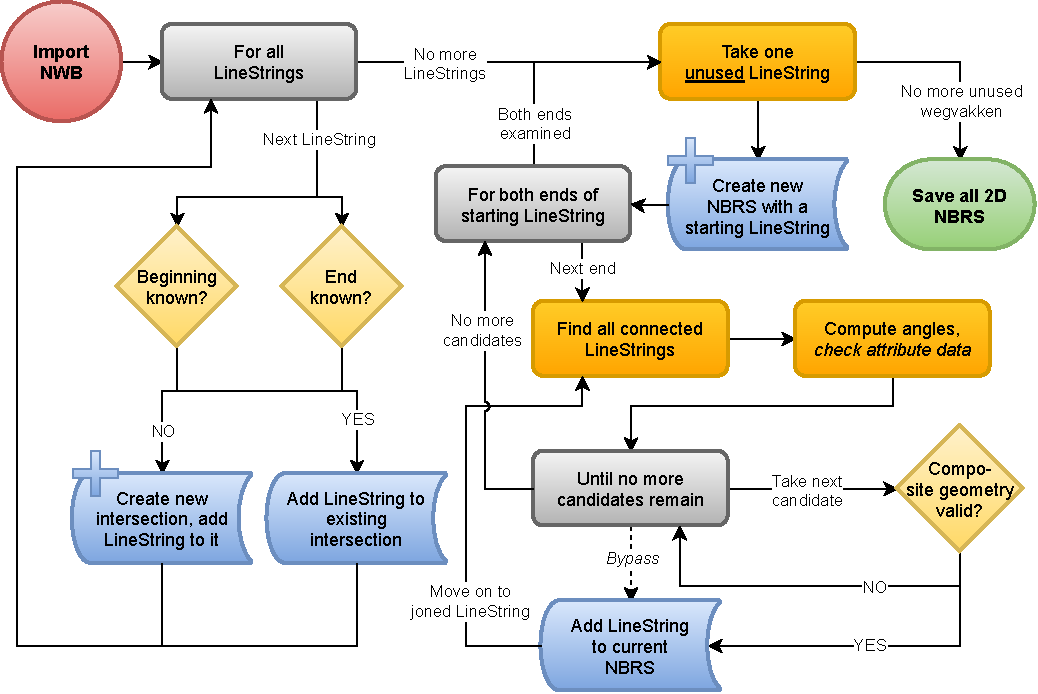
\includegraphics[width=0.9\linewidth]{final_report/figs/nbrs_generation.pdf}
    \caption{Flowchart-style illustration of the NBRS generation step of the pipeline.}
    \label{fig:nbrsgenerationflow}
\end{figure}

\subsubsection{Geometric algorithm}

This algorithm first creates a navigation structure from the input wegvakken. Each wegvak is a valid LineString, i.e. a connected series of line segments, which can be a few metres long, or even tens of metres long. From here on in this section, I will refer to wegvakken as LineString objects to make the description more general. The navigation structure is essentially a database that records which LineStrings of the road network start and end in which intersections. As this algorithm is not allowed to use the pre-made NWB intersections from the attribute table, intersections are defined by their coordinates (to one decimal). The navigation structure is based on hashing, hence it has good performance. The procedure consists of examining both ends of each input LineString and either creating a new intersection with it (if one does not exist at that location yet), or adding a reference to it in the intersection that is already found in the navigation structure. This is shown on the left in Figure \ref{fig:nbrsgenerationflow}.

The next step is to iteratively nucleate NBRS generation until no unclassified LineString objects remain. The algorithm takes one LineString, initialises an NBRS with it, and then attempts to extend it with further LineStrings on both ends to form an NBRS. First, recursive extension is initiated on the last vertex of the LineString, and once that completes, on its first vertex. The recursion examines the vertex, uses the navigation structure to find connected LineStrings and may connect one of them if certain conditions are met (see the next paragraph for the conditions) and progresses deeper into the recursion by doing the same with the LineString it just connected.

When the search for connected LineStrings succeeds, either a single one may be found, or multiple ones in case of a real-life intersection. If multiple candidate LineStrings were found, the algorithm needs to decide which one to connect based on a set of geometric conditions. First the angle between the last line segment of the previous LineString and the first line segment of all the candidate LineStrings are examined, and the continuation with the most optimal angle is selected (corresponding to the straightest possible continuation of the road). A composite geometry of the pre-existing NBRS and the new segment is then created and tested for self-intersections. If the composite geometry fails this test, the next best candidate is examined, and so on until a candidate succeeds, or the iteration runs out of candidates in which case the recursion terminates. When both recursions (going forward and backward from the LineString that nucleated the NBRS) finish, the NBRS is deemed complete and the next NBRS is nucleated. The self-intersection test is also performed when only one connected LineString is found.

\subsubsection{Semantic algorithm}

The semantic algorithm is built on the same framework as the geometric one. Most steps of the procedure are slightly modified equivalents of the ones in the geometric algorithm, hence I will here focus on describing the differences.

The navigation structure of the semantic algorithm is based on the JTE IDs (junctie IDs) found in NWB, which are unique identification codes belonging to each intersection of wegvakken in the dataset. Each wegvak possesses an end and beginning JTE ID, which are used to assemble the navigation structure in place of the coordinates in the geometric algorithm.

The nucleation of NBRS takes place in a similar manner to the geometric approach, but here each NBRS is associated with a specific wegnummer (road number) and BST code (a code related to the role of each road). LineStrings are only joined to an NBRS if they have matching road numbers and BST codes, which is what the text \textit{check attribute data} in the flowchart refers to. The candidates are still processed in the order or decreasing angle optimality, like in the geometric algorithm. However, the composite geometry needs not be checked for self-intersections, as roads satisfying the semantic conditions do not self-intersect in real life. This improves performance, as the intersection and validity checks of the resulting geometry is costly in terms of computational complexity. This shortcut is indicated by the dashed \textit{bypass} path in Figure \ref{fig:nbrsgenerationflow}.

\subsubsection{Challenges encountered}

I encountered three distinct issues while I was developing this part of the software. The first problem was that while NWB has a valid graph structure when one looks at its attribute table, the same graph structure is not always easy to derive solely from the geometry. While the semantic algorithm does not suffer from this problem, the geometric one does. Each wegvak has a pointer in its attribute table to the IDs of the two intersections it is connected to. This makes it possible to navigate the graph with minimal effort, but the underlying LineStrings may occasionally be disjoint (due to the coarse georeferencing NWB uses), in which case the software needs to "guess" which other LineString it might be connected to, if any. Fortunately, this was not difficult to implement using the coordinate-based navigation structure - reducing the decimal precision in it solved the issue in most places. A second issue was that the geometry of wegvakken often reverses in the middle of a valid series that might form an NBRS, requiring the implementation of a workaround especially in the code that computes the angles. Lastly, for reasons that have to do with external conditions that NWB needs to meet, motorway ramps are connected to motorway lanes at angles that do not reflect real-life geometry, occasionally causing the algorithm to merge ramps into motorway NBRS and vice-versa. A dedicated workaround was also necessary here, to recognise this situation and treat it correctly.

\subsection{Elevation estimation}
\label{sub:m_elevationestimation}

The elevation estimation stage of the pipeline consists of two operations. The first operation is to associate each NBRS vertex with a preliminary elevation estimate based solely on nearby Lidar points, and the second a refinement step to eliminate occlusion-related artefacts. The procedure is illustrated by the flowchart in Figure \ref{fig:elevationestimationflow}.

\begin{figure}
    \centering
    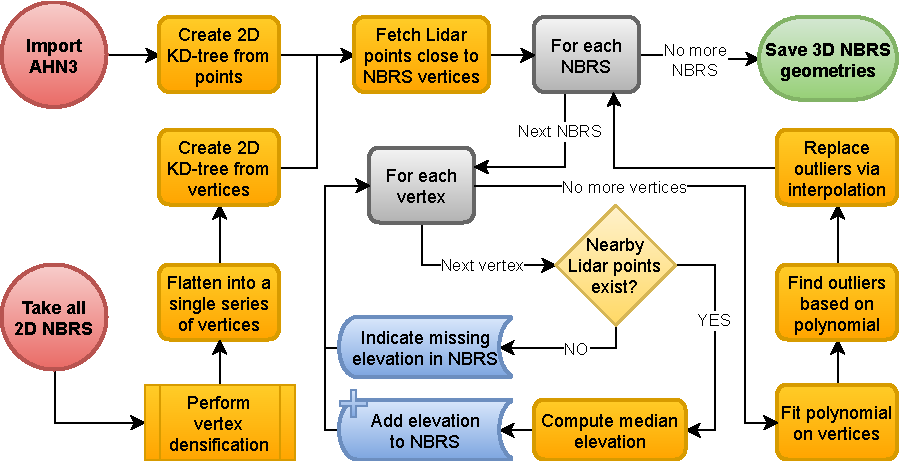
\includegraphics[width=0.9\linewidth]{final_report/figs/elevation_estimation.pdf}
    \caption{Flowchart-style illustration of the elevation estimation step of the pipeline.}
    \label{fig:elevationestimationflow}
\end{figure}

\subsubsection{Initial elevation estimation}

The process starts by importing AHN3, from where elevations will primarily be derived. It is assumed that this input is sufficiently small to allow in-memory use, i.e. that it is a cropped or clipped version of the full point cloud tile. Thus, this is the point in the procedure, where a global scaling solution would be most important. All other parts of the program work on the basis of processing subdivisions of the road network (NBRS or the underlying LineStrings themselves), which is already a good starting point for scaling.

The imported point cloud is first converted into a 2D KD-tree, so that area-based queries can be performed efficiently on it. This is followed by the flattening of all NBRS vertices into a single series, which was implemented in an effort to improve performance. Sending all vertices into the KD-tree query program at the same time as a flat list of vertices is far more efficient than performing the query individually for each NBRS vertex. This approach is reused in many subsequent parts of the implementation. Points closer than a certain threshold distance are fetched for each NBRS vertex. Before elevations are estimated, the flat list of coordinates is first split back into the discrete 2D profiles that NBRS represent. The median elevation of the nearby Lidar points of each NBRS vertex is then computed as a representative elevation estimate. Where too few points where found, the elevation is instead marked to be missing.

\subsubsection{Refining the preliminary elevations}

Following this step, each of the thus 3D-enriched NBRS are fed into an outlier filtering algorithm. The algorithm generates a distance series based on the horizontal coordinates of the NBRS, and fits a polynomial on these distances, and the elevation estimates. Since occlusion is almost always represented by short-wavelength data gaps or positive outliers in the Lidar data, these vertices will have considerable errors relative to the fitted polynomial. By interpolating values where outliers were detected and where elevations could not be obtained prior to this step, the quality of the preliminary elevations is improved considerably. The steps of this procedure are shown on the right in Figure \ref{fig:elevationestimationflow}.

The replacement values for outliers are interpolated \textit{linearly} based on the series of inlier vertices, i.e. they are not determined by the polynomial fit. The reason for this is, that it is not always possible to find good fits for NBRS using a fixed-degree polynomial, and while the polynomial model is always good enough to \textit{detect} outliers, its values are not conformant enough to replace them with. This polynomial-fitting approach is reused in various subsequent parts of the implementation.

The resulting coordinates now represent smooth 3D lines that preserve the input road network's 2D georeferencing, but which were enriched with elevations. These series are retained both as a list of vertices for the convenience of subsequent steps, as well as updated geometries of the original LineStrings that comprise the input road network. At this point, a preliminary 3D version of the road network can be written to disk.

\subsubsection{Vertex densification}

Although it is not strictly related to NBRS generation, vertex densification is not listed as a discrete pipeline step as it is a rather trivial operation conceptually. As a result, it is only presented in this report as a pre-processing operation of the present step of the pipeline. It is shown in \ref{fig:elevationestimationflow} as the first processing step that acts on 2D NBRS.

Vertex densification of the NBRS vertices refers to the operation of taking the wegvakken that make up each NBRS, and adding vertices to their line segments until no distance between vertices is bigger than a certain threshold. In my implemetation, this takes place as a recursive iteration. Each wegvak (LineString) of each NBRS is considered, and the densification algorithm is called on each line segment. The recursion consists of breaking the line segment in two halves if it does not comply with the threshold (a vertex is added in the middle), and then proceeding deeper into the recursion by doing the same with the two resulting halves. The densified geometries are assembled when returning from the frames opened by the recursion.

Like NBRS generation, vertex densification is done for the benefit of subsequent operations. Many operations - such as the present step - act on each vertex separately, gathering information related to the vertex from its AHN3 and DTB neighbourhood. Since the posting distance of AHN3 is far smaller than the line segments in NWB, increasing the density of NWB's vertices has practical benefits. It not only increases the resolution at which elevation can be estimated, but it also means that large-scale trends in the data will be represented more dominantly, i.e. algorithms will be better able to tell which parts of the road represent the road surface, and which ones are outliers due to occlusion. The practical benefits of this step were observed during development, and vertex densification was made an intrinsic part of various other parts of the pipeline too.

\subsubsection{Challenges encountered}

The main challenge encountered was that at the beginning of the algorithm, NBRS still consist of references to a series of wegvakken (LineString objects), but which then need to be flattened into a single series (for KD-tree queries). Thus, the problem regarding random reversals of wegvakken still stands, and a workaround needed to be implemented that rotates reversed wegvakken into the correct orientation during the flattening step. The correct orientation is always relative to the first wegvak in the NBRS. Needless to say, these then needed to be rotated back again into their original positions when writing the elevations into the source data, to avoid introducing changes to the 2D geometry of NWB.

A second challenge was to find a good benchmark of what to consider outliers after fitting polynomials. I needed to choose a metric that works well with all the typical types of occlusion-related artefacts that might show up in the data, such as overlying bridges of various heights, civil engineering structures of such bridges next to and above roads, motorway signs, tunnels, and so on. After experimenting with various approaches, I settled on one that involves computing the standard deviation of errors relative to the polynomial model, and then setting the threshold as a multiple of standard deviations (which is also in line with standard scientific practice). Below a certain absolute value of standard deviation, I artificially raise it to a set minimum level to avoid performing interpolation in road surfaces that are exceptionally smooth.

\subsection{Lidar segmentation}
\label{sub:m_lidarsegmentation}

The Lidar segmentation workflow is more complex than the two I described above, and some of the intricacies are omitted in the relevant flowchart (Figure \ref{fig:lidarsegmentationflow}) to keep its complexity manageable. I will attempt to fill in some of these details here in the text, referencing where approximately in the flowchart they occur.

\begin{figure}
    \centering
    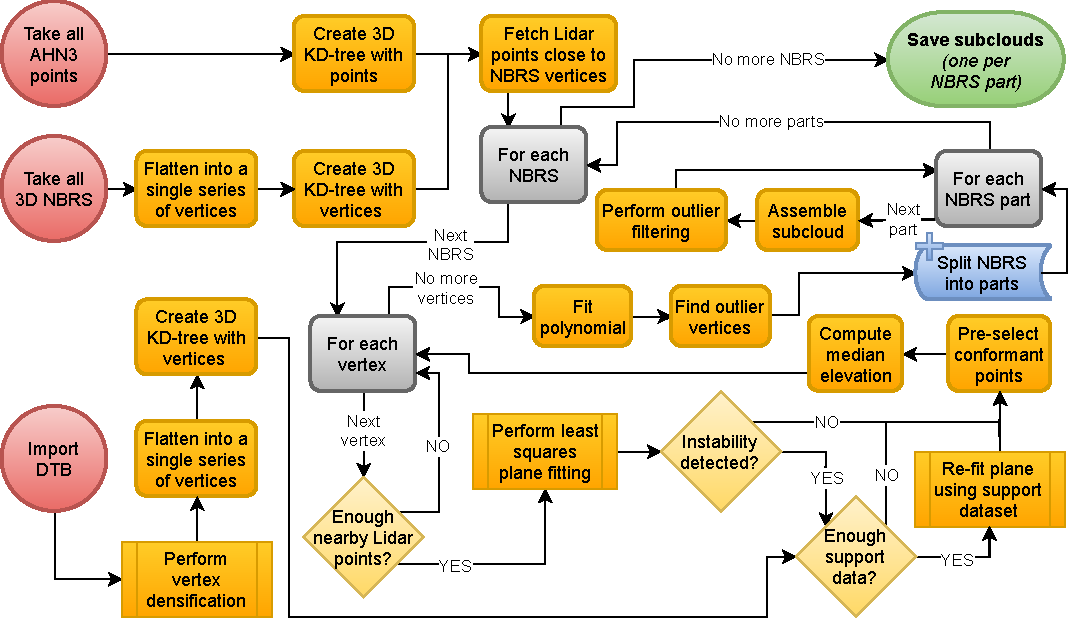
\includegraphics[width=0.9\linewidth]{final_report/figs/lidar_segmentation.pdf}
    \caption{Flowchart-style illustration of the Lidar segmentation step of the pipeline.}
    \label{fig:lidarsegmentationflow}
\end{figure}

\subsubsection{Preparation and plane fitting}

The program first creates KD-trees from the 3D point cloud, the flattened list of all 3D NBRS vertices, as well as a flattened list of all vertices found in the support dataset, DTB. Since DTB is a vector dataset that consists of 3D LineStrings, the lines are also vertex-densified prior to being converted into a point cloud and then into a KD-tree. The densification drastically increases the effectiveness of using DTB as a point cloud.

Much like in the preliminary elevation estimation workflow, a Lidar point cloud KD-tree query is performed as a bulk operation on each NBRS vertex (using the KD-tree made from the NBRS vertices). This results in "patch" of Lidar points being selected for each NBRS vertex with the underlying selection geometry being a sphere, rather than a 2D circle (as was the case in preliminary elevation estimation). This means that the relevance of the selected points will already be far more certain than before. However, each of these patches are further processed below to enhance the results.

The program then fits a plane on each patch of Lidar points using the least-squares method. Planes are only fitted if there are a set minimum number of points to support it, a threshold which is defined in terms of reaching a certain minimum point density inside the patch. If it is not reached, the points may still be passed on if a lower threshold is reached, in the hope that the support dataset (DTB) can re-position the plane to them in later parts in the algorithm and find some of them to be conformant with it. Below this second threshold, neither a fitted plane, nor the points are passed on. In the flowchart (Figure \ref{fig:lidarsegmentationflow}), this stage is shown in a simplified form which excludes the logical branch between the two thresholds, as it is insignificant.

\subsubsection{Refining plane fits and pre-selecting points}

Next, the program processes each NBRS starting from their first vertex and considering each vertex, one by one, in the order in which the vertices geometrically represent the road centreline making up the current NBRS. The program searches procedurally for places where the succession of fitted planes may indicate a break in shape of the surface. At the beginning of the iteration, the program first initialises a set of variables describing the \textit{previous} plane fit's relative position to the 3D NBRS centreline, the median elevation of the relevant patch's Lidar points, and the standard deviation of their distances to the fitted plane. By examining variations in these metrics (comparing always those of the current vertex and plane to the previous one), the algorithm can detect where the plane fits become unstable. Significant changes relative to the previous vertex and plane may indicate the presence objects occluding the sensor's view of the road's surface. I determined the exact metrics and parameters (thresholds) related to detecting instability based on experimentation and iterative refinement. The current setup works well with all testing datasets examined. This step is represented in the flowchart by the conditional element labelled "Instability detected?".

Originally, the algorithm was configured to automatically revert to the previous plane in case of plane instability and be allowed to use the reverted plane for a few iterations before asking help from the support dataset (in case the road emerged from underneath the occluding object after a few iterations). If the support dataset could also not help (due to e.g. a lack of coverage) after the expiration of the tolerance period, the algorithm would "give up" and move on to the next NBRS. This meant that long occluding objects and no DTB coverage could prevent the algorithm from processing certain NBRS, for instance ones containing tunnels.

\subsubsection{Handling breaks in the trend and missing data}

I eventually revised this algorithm to be more robust and to produce useful results even in a complete absence of a support dataset such as DTB. In the current version of the implementation, the algorithm is only allowed to attempt to use the previous plane \textit{once} before trying to use DTB. The point cloud generated from DTB contains road surface measurements only, so it can be relied on to provide "assistance" where AHN3 is ambiguous. If a previous valid plane exists, then DTB is queried for points relatively close to the previous valid plane (using the centroid of the points on which the plane was fitted). If not, then the centre of the query is the current NBRS vertex itself. If a reasonable amount of DTB points could be thus recovered, then the process is repeated by performing a second KD-tree query on the centroid of these DTB points, and the plane is then re-fitted onto the retuned points. The second query ensures that as many useful DTB points are included as possible. The program then assesses the distribution of Lidar points in the patch close to the re-fitted plane, and if the majority are found to be roughly conformant with it, then the plane is re-fitted a third time to make sure that in the end it is based on the Lidar points and not the support data wherever possible. The necessity of this last step will be reasoned in more depth in Section [REF], in a nutshell the reason in the case of my datasets was that in many places DTB is up to two decades older than AHN3, leading to significant, but locally consistent differences between the elevations suggested by the two datasets.

In the new version of the algorithm, the program does not declare failure if it is no longer allowed to revert the plane to the previous and find support data to also be unreliable or missing altogether. Instead, it simply relaxes its conditions and continues as though it were starting to process a new NBRS. This bypass allows the program to continue processing the NBRS even if it is aware that there was a noticeable shift in the position of the fitted planes, or a data gap. Artefacts due to such places are now handled separately, after the iteration has finished.

Each iteration of this algorithm finishes by looking at the final plane fit of the Lidar patch of the current vertex, and pre-selecting those AHN3 points which conform well with it. The median elevation of these points is also saved as it will be used in the next step. DTB points are also merged into this subcloud, but only in places were they were used to re-position the plane fit as described above.

The above iteration is shown as the loop labelled "For each NBRS vertex" in Figure \ref{fig:lidarsegmentationflow}. In the implementation, the nesting of the iterations in different, but this description is easier to understand and is fully equivalent to the implemented version in terms of what it achieves. The same is true about the top-level iteration ("For each NBRS" in the flowchart), which in the implementation is broken into several parts for programming convenience.

\subsubsection{Breaking NBRS into parts}

Once the last vertex of the NBRS has been processed, a post-processing procedure is executed before moving on to the next NBRS. Based on the median elevations which were saved during the iteration, the program once again has a new 1D profile which it can examine for outliers. Missing elevations in the series generally indicate that there is a data gap in both AHN3 and DTB there. On the other hand, outlier elevations almost always indicate that the plane fit was corrupted by an overlying features that caused occlusion or partial occlusion and it was also not possible to rectify the plane fit based on DTB. Instead of interpolating at these locations, the program generates a boolean mask. This boolean mask is then post-processed to eliminate short-wavelength changes and used to construct a list of intervals inside the NBRS that were found to be affected by neither of the above two problems. Thus, a further subdivision of the road network is introduced: \textit{NBRS parts}. Each part corresponds to an interval in its parent NBRS with reliable input coverage.

For each NBRS part, the patches are combined into a subcloud (including points which originate from the supporting dataset, in our case DTB). A quick outlier filtering step is applied to them eliminating all points in the subclouds which are isolated (have no neighbours within a certain distance). This is easy and computationally efficient to execute by converting the data into KD-trees and performing nearest-neighbour queries on them.

A hashed structure is initialised at this point in the program that allows the program to remember which points in the subclouds originated from the support dataset. The use of this structure is described in Subsection [REF] below.

As Figure \ref{fig:lidarsegmentationflow} shows, this concludes the point cloud segmentation procedure. Each NBRS part has its own subcloud, which are aggregated (but not merged) on the NBRS level and used in all subsequent parts of the program. The results can be written to disk as a LAS file, in which points are classified based on which dataset they come from, and which NBRS and NBRS part they belong to.

\subsubsection{Challenges encountered}

The above description already contains an account of how my methods relating to treating breaks in the trend and missing data evolved, and I will further elaborate here on this topic as it represents the biggest challenge encountered. While detecting small-scale variations in a range of metrics is not a difficult task in general, finding a set of metrics and corresponding thresholds universally applicable to all the data proved to be challenging. Furthermore, the simple approach of starting on one end of the NBRS and examining its vertices one by one eventually turned out to have insurmountable limitations. As it has no concept of global trends in the NBRS, it can only rely on its previous iterations to detect breaks in the trend. With the right configuration of metrics, I expected to be able to overcome this barrier, and wanted to keep this approach also because it allowed me to make use of DTB in an effective, elegant manner.

However, I eventually realised that this approach has another limitation: in regions with outlying or missing AHN3 data and no DTB coverage \textbf{and} a change in the elevation of the road, the iteration would lose its references and not be able to continue after the road emerged at the changed elevation. This limitation only manifested itself in places where NBRS contain long tunnels. Furthermore, keeping regions with no coverage inside NBRS also meant that in subsequent steps, I was optimising contours and continuing the road surface model TINs across them as well - sometimes over tens of metres or more. This turned out to be problematic especially with active contour optimisation, which frequently ended up producing corrupted outputs as a result.

To solve all these issues, I extended this part of the implementation with methods to examine the global trend represented by pre-selected points after the procedural iteration. This is where I transitioned to first saving Lidar patches per vertex separately (instead of adding them straight to the subcloud), constructing a polynomial based on their centroids to describe the overall trend, and detecting areas where the points lay above the expected road elevation (converting these into no-data regions). Then, all I had to do is break NBRS into parts where such no-data regions begin and end, and propagate these changed to all the subsequent parts of the pipeline. As this step takes care of outlier planes where no DTB coverage is available, the role of the procedural iteration was reduced to managing DTB-based filling of holes, it no longer tries to eliminate outlier patches on its own, where DTB is unavailable.

\subsection{Edge approximation}
\label{sub:m_edgeapproximation}

The generation of preliminary edges is based on identifying edge points at discrete intervals in the road centreline (on each vertex, including ones created during vertex densification). The procedure takes place on the level of NBRS parts, and it is illustrated in Figure \ref{fig:edgeapproximationflow}.

\begin{figure}
    \centering
    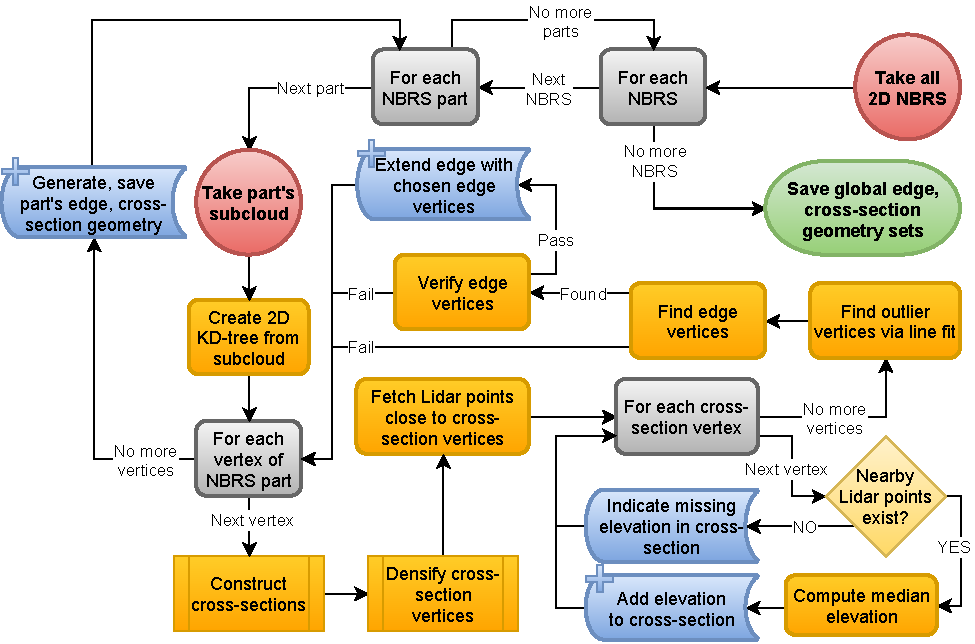
\includegraphics[width=0.9\linewidth]{final_report/figs/edge_estimation.pdf}
    \caption{Flowchart-style illustration of the edge approximation step of the pipeline.}
    \label{fig:edgeapproximationflow}
\end{figure}

\subsubsection{Constructing edge point candidates}

First, the subcloud of each NBRS part is used to create a 2D KD-tree. 2D suffices here, because it is a reasonable assumption to make at this point that the subclouds of NBRS parts no longer have a significant number of points that would not describe a 2.5D surface (e.g. reflections from occluding objects). On each vertex of the NBRS part, a cross-section is then constructed. Cross-sections are built roughly orthogonal to the centreline locally, their azimuths are based on the mean azimuths of the two line segments that contain the given vertex (except for the first and last vertices, which are simply based on their single parent segment's azimuth). The cross-sections are densified considerably and their densified vertices' are then flattened into a single list and used in a bulk KD-tree query. Lidar points very close to the vertices are thus fetched, and their median elevation is saved as the elevation of the given vertex. This step works on a small, sub-metre scale, meaning that using the native density of AHN3 (no thinning applied) is particularly important from here on.

Each cross-section then represents a 1D profile, elevations against distance from one end to the other (with the NBRS part's vertex in the middle). Each of them is fitted with a line and outlier vertices are identified based on the model line. The program then tries to find suitable edge points among the inlier cross-section vertices, on both sides of the NBRS vertex in each cross-section. Together, these points will form the preliminary edges. In each of the cross-sections, the program starts from the outermost cross-section vertex and progresses inwards. Once a certain consecutive number of inliers is encountered with no outliers in-between them, the program assumes having reached the road surface and flags the current vertex as the edge vertex.

The full length of each cross-section, which is a constant parameter, represents the maximum road width the program can work with. The optimal value of this parameter depends on the permitted road dimensions in the given road network (AHN3 in our case), and it lies in a rather narrow band. If it is too small, the preliminary edges may lie far inwards from the real-life edges, and exclude large portions of the real-life road surface as a result. If it is too large however, false positive hits outside the real-life road surface will corrupt the preliminary edges, especially where roads are thin and other smooth surfaces are found in their surroundings.

\subsubsection{Enforcing constraints}

Flagged vertices are only accepted as edge vertices if they also pass a range of further conditions relating to the minimum width, as well as sudden elevation changes and road width changes. The minimum road width is enforced for each pair of edge points individually. However, much like in the first part of the Lidar segmentation step, the latter two are checked by comparing the metrics of the current edge point candidates to a previous few. Only if this verification procedure succeeds, does the program extend the NBRS part's preliminary edges with new vertices.

In areas where the above procedure fails multiple times consecutively, "gaps" are created in the preliminary edges. These are not real gaps in the sense that the last pair of edge points before the gap, and the first pair after, are still connected in the output - it simply means that the lengthwise sampling is coarser locally. Compared to the artefacts that would appear in the absence of the above threshold enforcement procedure, small gaps are an acceptable compromise, especially if the NBRS were sufficiently vertex-densified prior to this step. However, long gaps cause various problems in later pipeline steps. To avoid creating long gaps in the generated edges, a relaxation of the conditions takes place after a set number of failures. After relaxing the conditions, the first inlier point is selected when fitting the next cross-section with a line, and the constraint regarding sudden changes in width is also ignored. Immediately after a success, the constraints are re-enabled. This temporary relaxation allows the algorithm to regain its reference even if a sudden real-life change in the road's width is encountered, and also helps in scenarios where the location of the edge is ambiguous.

Lastly, once per NBRS part the program generates the final 3D cross-section and edge geometries and saves them. After all NBRS parts have been processed, the global cross-section and preliminary edge object is also created. This can be written to disk as a Shapefile to visualise the results.

\subsubsection{Challenges encountered}

Originally, this step was going to be a preparatory step for the sole purpose of providing initial edge shapes for the active contour optimisation algorithm. I first implemented it almost exactly to the specifications found in the P2 document. However, it soon became clear that better active contour optimisation results require better preliminary edge estimates, and thus I implemented a range of tweaks and improvements. It appeared that the best active contour optimisations corresponded to where the preliminary edges were on the road surface, slightly inwards from the location of the real-life road edges. This is what defines the final implementation of picking edge point candidates - the program starts from the outer edges of the cross-sections, and progresses inwards until it can safely conclude that is has already been inside the road surface for at least a few vertices.

A further challenge corresponded to the point in development when I decided to make active contour optimisation optional. I needed to implement modifications to these methods to allow preliminary edges to be used for TIN construction directly, at the same time still maintaining compatibility with active contour optimisation. This is what resulted in the addition of the system of constraint enforcement and constraint relaxation that takes place right before accepting a pair of edge point candidates. The main reason why this is beneficial for TIN construction is that it ensures that the edges do not have a zero (or very tiny) width anywhere, and that it reduces the chance of road widths being overestimated. The former ensures that there is always a non-zero area on both sides between the underlying road centreline and the corresponding preliminary edges, in turn ensuring the possibility to select Lidar points in these 2D areas in the TIN initialisation step. The latter decreases the chances of including off-road points in the road surface models, both during TIN initialisation and extension. For more information about the TIN construction phases, please refer to Section \ref{sub:m_tinconstruction}.

\subsection{Active contour optimisation}
\label{sub:m_activecontours}

The optimisation of preliminary edges is based on constructing one attractor map for each NBRS part, and running active contour optimisation to attract the preliminary edges to certain features in the attractor maps. The procedure is illustrated in Figure \ref{fig:edgeoptimisationflow}.

\begin{figure}
    \centering
    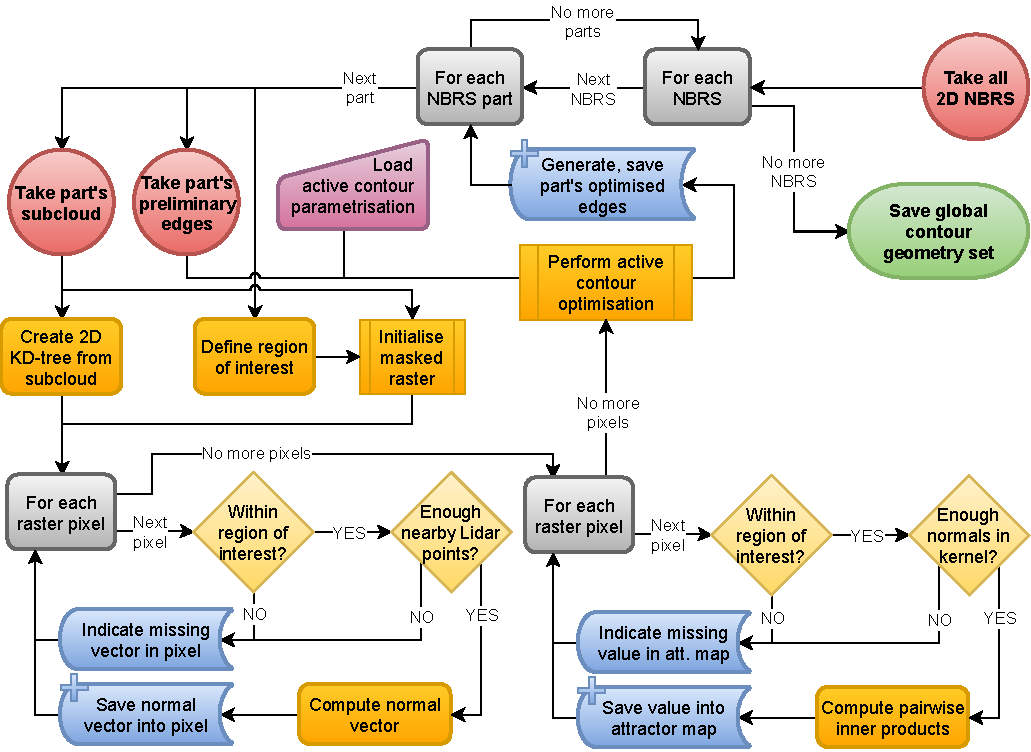
\includegraphics[width=0.9\linewidth]{final_report/figs/edge_optimisation.pdf}
    \caption{Flowchart-style illustration of the active contour optimisation step of the pipeline.}
    \label{fig:edgeoptimisationflow}
\end{figure}

\subsubsection{Attractor map generation}

The procedure underlying this step is once again based on a 2D KD-tree of the subcloud of the NBRS part. 2D suffices because the underlying data structure of attractor maps are 2D rasters, and once again, because we are safe to assume at this point that the subclouds of NBRS parts no longer have a significant number of points that would not describe a 2.5D surface. When initialising the raster that underlies the attractor map, a region of interest is first derived by buffering the centreline by a certain amount. The rectangular-shaped raster is then masked out everywhere except for pixels whose centres lie within the region delineated by the buffer polygon.

The centre of each unmasked pixel is then used in a bulk KD-tree query to find a small 2D patch of nearby Lidar points. For pixel centres that have a sufficient amount of neighbouring Lidar points, a normal vector is computed. These normal vectors are computed as the normal vectors of the local plane fits of each such patch of Lidar points, and the least-squares-based approach is re-used in my implementation (from the Lidar segmentation step of the pipeline).

Normal vectors can be stored in the pixels in my framework, but they cannot be used directly in active contour optimisation because it requires scalar pixel values. To derive scalar values from the vectors, I designed a kernel-based approach in which the pairwise inner products of the normal vectors of all pixels falling into the kernel are computed and their median is taken. Since computing inner products is computationally expensive, not all combinations of the normal vectors in the kernel are dotted, only a representative random subset.

\subsubsection{Running the optimisation algorithm}

All parts of the above procedure take place in a temporary coordinate system which is defined in terms of the number of pixels in the X and Y dimensions from the top left corner. Before the preliminary edges can be overlain on the attractor map, they each need to be transformed into this coordinate system via scaling and translating their coordinates. Together with the attractor maps and a suitable parametrisation, the preliminary edges are now ready to be optimised. The optimisation algorithm is run separately for the edges on the two sides of the centreline, and the output optimised edges are then assembled into a single polygon (the NBRS part's contour). Lastly, the global collection of contours are assembled into a single object which can be written to disk to visualise the results.

The scikit-image implementation of active contour parametrisation is based on the original paper in which this this method was first described scientifically: \cite{kass_etal_1988}. In addition to taking the attractor maps and the preliminary contours as input, it also takes a set of parameters that can be tweaked to manipulate aspects of the optimisation. The most important aspects for us in this project are contour smoothness, attraction to brightness, attraction to edges and the total number of allowed iterations.

In Section [REF] I describe the recommended values for each of the variables, based on the fine-tuning I carried out as part of implementing this step. Here, I will describe the aims I had in mind while fine tuning. Firstly, the $\alpha$ parameter is set to zero in order to prevent the contours from contracting. Shrinking the contours lengthwise is not desired, as it needs to extend all the way to the two ends of the underlying NBRS part. Medium smoothness is desired because based on the testing I have done, this is one task in which active contour optimisation excels, it can smooth preliminary edges in a way that can eliminate small-scale protrusions that are generally meaningless, and can thus be considered noise. Importantly, I was unable to make use of the ability of active contour optimisation to take into account brightness. The attractor maps that I described above have a sharp contrast between the brightness of off-road pixels (which are dark), an road pixels (which are bright). However, this contrast is not localised to the edges of roads, hence any amount of attraction to either region would draw the contour deeper into that region rather than keep it on their boundary. Attraction in my recommended parametrisation is controlled entirely by edge detection, as this works correctly with my attractor maps. In terms of iterations, I decided to work solely with a maximum number of iterations rather than reaching a certain boundary condition. Setting a boundary condition terminates the optimisation process when the contours no longer move significantly in each step. Unfortunately, letting the contours evolve to this point results in the drastic enlargement of artefacts, as well as an unacceptable increase in computational complexity - I found iteration limits between 100 and 5000 to be the most effective, with each iteration being permitted to move the contour by up to one pixel only.

\subsubsection{Challenges encountered}

In terms of the first version of my implementation, the main challenge here was the trial-and-error nature of getting active contour optimisation to perform acceptably for the wide range of input geometries and attractor map features that are possible in our national datasets. I needed to refine the parameters of the optimisation algorithm needed to work well with the input data, but since I was also producing the input data myself, I was also in the position to fine-tune that in turn. As a result, the task was a joint fine-tuning procedure involving all prior steps in the pipeline leading up to this point, as well as the arguments in the algorithm's API. Of all the aspects of the input data that I tried to optimise, I invested the greatest amount of effort in pre-processing the attractor maps to bring out the the road edges in them as sharply as possible. I tried various moving-window techniques such as many types of edge detection, edge enhancement, blurring, as well as morphological operations such as dilation, erosion, opening, closing, and many combinations thereof. Sadly, I eventually concluded that none of these operations can achieve a noticeable improvement in the results, with the kernel-based normal vector attractor map and the native edge detection of active contour optimisation still producing the best results after several days spent on this.

Making matters worse, I found active contour optimisation to work only at high raster resolutions, with a pixel size around 0.5 metre typically producing the best results overall. Unfortunately, computational complexity grows non-linearly with decreasing pixel size, making debugging and fine-tuning very difficult, as well as putting the usefulness of such an algorithm into question considering the scale of the input data.

A further problem I found is that there are occasional small-scale features in the input data that tend to confuse active contour optimisation. Even for relatively short iteration lengths, such small artefacts may unpredictably corrupt entire NBRS part contours. For instance, small Lidar gaps due to stationary vehicles frequently overlap with the region where the road edges are suspected to be found. Active contour optimisation has no concept of no-data pixels, and reacts unpredictably to these holes regardless of what one uses as filling values. Another similar issue is that road edges are often characterised by sudden slopes beyond their edges, but with further flat regions beyond them. These slopes are often short, and their intersection with the off-road flat zone creates a second contrast in brightness that active contour optimisation may confuse with the real road edge. These features and other similar types of features frequently draw the contours further from the road than what would be acceptable to accurately classify Lidar points within the contours as road reflections.

Lastly, the effectiveness of the method is also far too reliant on the accuracy of the preliminary edges. The algorithm is sensitive to even the smallest of blunders in preliminary edge detection, and is also prone to fail in no-data regions. After I implemented the code to split NBRS internally into parts where longer regions suffer from the absence of data, part of this issue was solved, but another remained: where DTB is available but not AHN3, preliminary edges tend to shrink significantly, which often corrupts the optimised edges.

While my implementation works and produces usable results, its ineffectiveness an unreliability prompted me do make it possible to bypass its use in the software. This required modifications to various preceding steps of the pipeline, as well as all subsequent ones - a significant challenge. This bypass in turn puts into question the relevance of much of the pipeline structure, many parts of which were intended to lay the groundwork for active contour optimisation, and to make use of its output. I elaborate on this topic further in Section [REF].

\subsection{TIN construction}
\label{sub:m_tinconstruction}

As I emphasised in the previous section, various aspects of active contour optimisation were found to be lacking. The severity of the issues with this step prompted me to develop TIN construction in a way that enables it to function without active contour optimisation. Bypassing  the active contour optimisation step alters the requirements that the TIN construction algorithm needs to satisfy. In my planned pipeline, I made the assumption that points falling within the area of contours could be safely considered road points, and that conditional insertions would primarily be used to filter out obvious outliers. Working with preliminary edges (as well as \textit{inaccurate} optimised edges) necessitates a less straightforward, but more robust implementation that is capable of recognising outliers on a much smaller scale. The result is an algorithm that borrows ideas mainly from region growing and ground filtering algorithms. In in-depth explanation of the algorithm is found below.

The outermost iteration loops over NBRS, and NBRS parts are iterated one level below. In Figure \ref{fig:tinconstructionflow} this is explicitly indicated as iterating over NBRS IDs and NBRS part IDs respectively. In contrast with previous steps in the pipeline, the centrelines themselves are no longer used, hence the change in notation. 

\begin{figure}
    \centering
    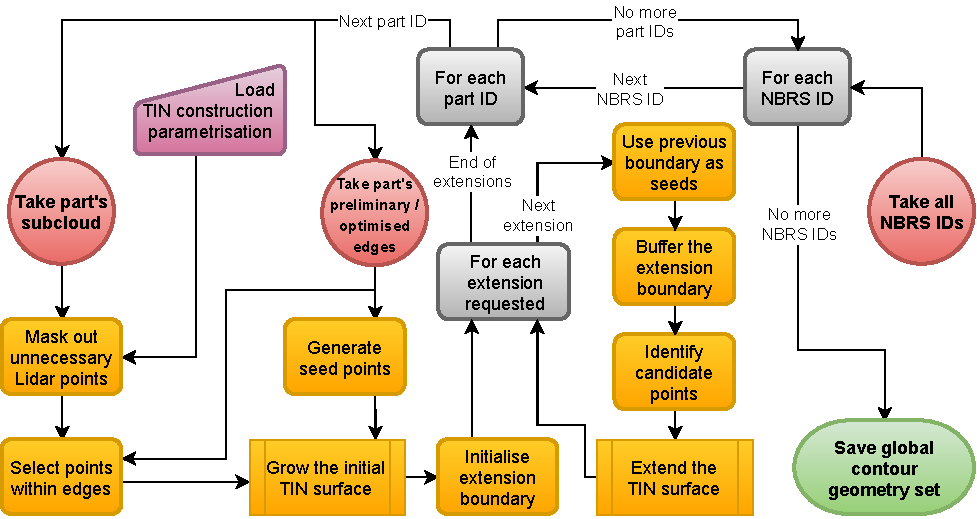
\includegraphics[width=0.9\linewidth]{final_report/figs/tin_construction.pdf}
    \caption{Flowchart-style overview of the TIN construction step of the pipeline.}
    \label{fig:tinconstructionflow}
\end{figure}

\subsubsection{Preparation for TIN initialisation}

Based on the parametrisation, the outermost boundary within which points will be considered for insertion (including TIN extension) is constructed as a polygon, and points falling outside of its interior are excluded from further consideration. Then, either the preliminary edges or the optimised edges are fetched for the given NBRS part. Since they are almost identical structurally, they can be treated the same way for the most part. They are used for two tasks: firstly, to construct a line halfway between the two edges to form the basis of seeding the TIN initialisation procedure, and secondly, to select points that fall within the edges as insertion candidates for the TIN initialisation step. This step is labelled "Grow the initial TIN surface" in Figure \ref{fig:tinconstructionflow}, marked as a pre-defined procedure because the underlying procedure is fairly complex. To keep the complexity of the flowchart manageable, both the TIN initialisation step, and the TIN extension step of this step are illustrated in a separate diagram, which is shown in Figure \ref{fig:tinconstructiondetailsflow}.

\subsubsection{TIN initialisation}

TIN initialisation refers to the process of constructing an initial, conservative approximation of the road surface. As I noted above, it considers those Lidar points only, which fall between the preliminary or optimised edges. It first looks up those Lidar points, which are very close to the seed points. As these points are all but guaranteed to fall on the real-life road surface, they are unconditionally inserted into the TIN and are then pushed on a stack that in this case I will refer to as the "buffer". At this point in the algorithm, as Figure \ref{fig:tinconstructiondetailsflow} shows, we leave the "TIN initialisation" group of operations and enter the "TIN growing" group (which is shared with "TIN extension"). The boundary vertices are also inserted into the TIN at this time (at an elevation of zero), which guarantees that the program can identify situations in which it is working with a triangle that touches the boundary.

At this time, the TIN contains a high density of small triangles in the immediate vicinity of the original centreline of the NBRS part. Furthermore, it contains large triangles connecting this area with the boundary inside of which the road surface is allowed to grow. During the initialisation stage, this boundary is represented by the preliminary edges or optimised edges themselves. Inserting these in the TIN serves a dual purpose. Firstly, it avoids raising errors when a conditional insertion test is being performed outside of the convex hull of inserted Lidar (and DTB) points. The boundary itself becomes the convex hull during the initialisation step, so each time the program tries to locate the triangle into which a given point would be inserted if it passed the test, will be guaranteed to succeed. Secondly, since the boundary is at an elevation of zero in the TIN, the program can easily identify when it is \textit{growing} the Lidar-defined surface rather than just inserting into a triangle already defined by three points from the subcloud. It also allows the program to be aware of the position of the tested point relative to the detailed surface and the boundary.

The buffer at this point consists of all the seed points that were inserted unconditionally. The buffer is fed into a KD-tree query over all the candidate points (points between the edges) in a bulk operation, and is then emptied. All points returned by the query are pushed on a stack, and this stack forms the basis for the conditional insertions. One by one, points on this stack are popped, and are conditionally inserted into the TIN. Figure \ref{fig:tinconstructiondetailsflow} does not describe the conditions themselves, but I will go into detail about them here.

First, the triangle containing the popped point is located. If the triangle is defined by subcloud points, then the elevation of the point according to the triangle is interpolated and the the difference in elevation is treated as an elevation discrepancy to which a threshold applies. If the threshold is not violated, then the distances to the three vertices of the triangle are computed, and based on that, the angles between the triangle's plane and the line segments connecting the popped point to the three vertices are also calculated. If any of the three angles violate a pre-set threshold, the point is not inserted.

If the located triangle contains one or more boundary points, the elevation discrepancy is computed in a different way. Growing the TIN needs to be done with some caution, as introducing erratic points around the edges of the current convex hull would entail that future insertions would have an incorrect basis for the conditional insertions and as a result, the surface would occasionally be allowed to grow in diverging directions. To minimise the chances of this happening, growing the surface takes into account multiple pre-existing TIN triangles in the neighbourhood, not just the closest ones. Specifically, all triangles containing the non-boundary vertices of the located triangle are fetched. Then, this is repeated with all the vertices of the resulting set of triangles. The vertices of this collection of nearby triangles are then fitted with a plane (re-using, once again, the least-squares method), and the distance of the tested point to the plane is taken to be a good approximation of the elevation discrepancy. Points in the buffer are always close to the pre-existing Lidar points in the TIN (see below for the reason), hence this is a reasonable assumption. The angle-based test is then administered the same way as for regular insertions.

Each popped point that ends up being inserted into the TIN is also pushed onto the buffer, which was previously emptied after it had been used for the KD-tree query to fill the stack. Once the stack becomes empty, the procedure restarts by performing another KD-tree query using the buffer, and refilling the stack with new points to insert conditionally. In other words, as long as points are being inserted, and these points have uninserted subcloud neighbours, the procedure will repeat. The buffer and the stack are kept separate so that KD-tree queries can be performed periodically as bulk operations, rather than individually - this is more efficient computationally.

As soon as no more insertions are taking place, the iteration ends and returns all points inserted into the TIN, in the order they were inserted. The TIN itself is not kept, instead it is reconstructed later on - this is due to the fact that point deletions in the triangulation package "startin" do not appear to work reliably, but we do not wish to keep the boundary points in the TIN. The straightforward way to achieve this without point removal is by reconstructing the TIN with the subcloud points only, keeping an external track of insertions to make this possible.

\subsubsection{TIN extension}

The extension of the TIN takes place in an iterative manner. The implementation accepts arguments that set the amount by which the boundary should be buffered in each iteration, as well as the number of extension iterations (steps). The starting boundary is \textit{not} the same as the one used during initialisation of the TIN. There, the preliminary or optimised edges were used, but here the first iteration's boundary is buffered from the seed line (the line halfway between the preliminary or optimised edges). This allows the algorithm to take another look at the points between the edges in case in missed any good candidates during initialisation.

The seeding of extension iterations is different than that of the initialisation step. The seed points are always derived from the boundary used in the previous iteration. Furthermore, in TIN initialisation the candidate points included all points between the road edges, whereas in the extension steps only the points located in 2D between the previous and the current boundary, are considered. Depending on the parametrisation, the boundary may be buffered to examine areas beyond the preliminary or optimised edges, which is the main point of the extension phase. It allows the program to grow the surface into areas which were not between the edges because of imperfections in how the edges were generated. It is, in a way, a means to counteract the phenomenon of the road surfaces getting very thin where edge detection or optimisation underestimated their width.

Each iteration first reconstructs the TIN yielded by the previous iteration, and inserts its new, buffered boundary into it. Boundaries are always at zero elevation, hence when the previous iteration's boundary is reused to seed the current iteration, it first needs to be \textit{transposed to 3D}. This is done by creating a KD-tree from all pre-existing TIN points and associating the closest one's elevation with each vertex of the seed geometry. It is then ready to seed the new iteration by itself being the basis for KD-tree queries on the new candidate points. However, the results of this query are not inserted into the TIN unconditionally, like they were in TIN initialisation. Instead, they are simply pushed to the buffer to start the main iteration involving the conditional insertions. The assumption that points close to the seed geometry are sure to be part of the real-life road surface no longer applies, as the seed geometry in extensions may be far from the centreline depending on what stage of buffering it is in.

Once TIN extension has finished, the final TIN is reconstructed and is saved. Thus, one TIN object per NBRS part is saved, and these are not merged or joined together into a single TIN in any way. My implementation offers the possibility to write these TINs to disk, each one in a separate OBJ file. The algorithm automatically filters out triangles with areas and circumferences large enough to indicate that they cannot be relevant to the road surface.

\begin{figure}
    \centering
    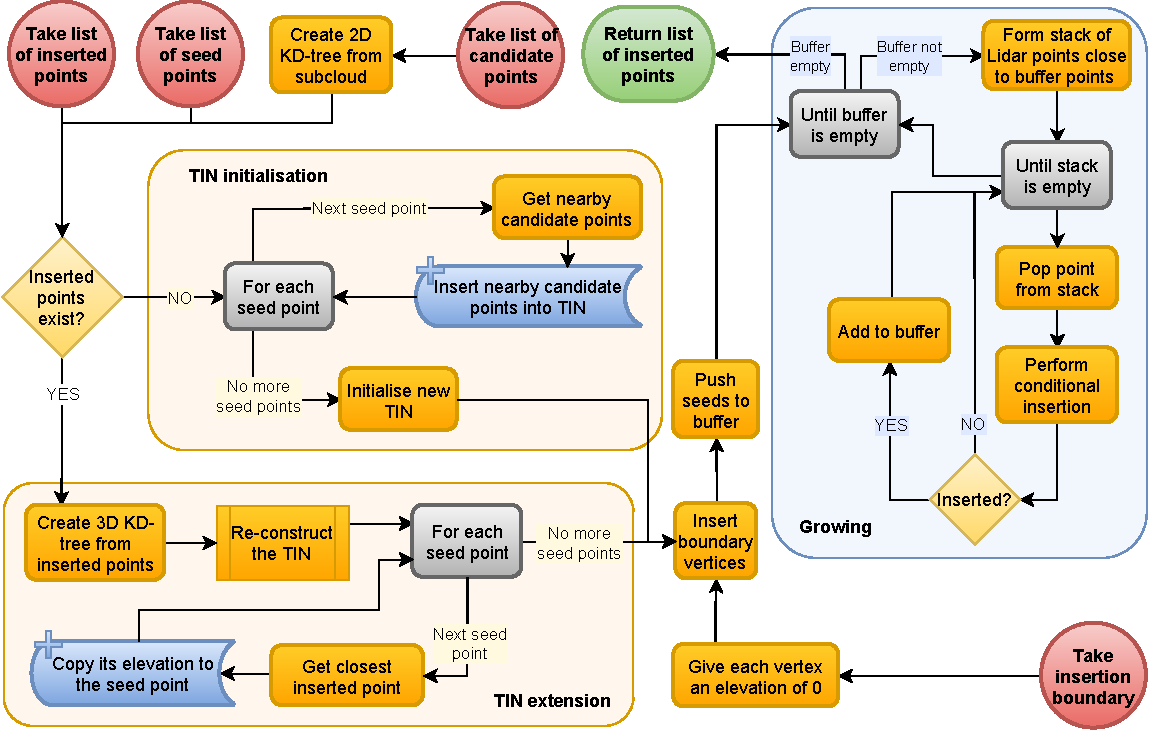
\includegraphics[width=0.9\linewidth]{final_report/figs/tin_construction_details.pdf}
    \caption{Flowchart-style illustration of the details of the TIN construction step of the pipeline.}
    \label{fig:tinconstructiondetailsflow}
\end{figure}

\subsubsection{Challenges encountered}

As implementing such a complex algorithm in this pipeline step was not originally intended, the biggest challenge here was to come up with a good solution within the timeframe reserved for the project. In terms of the methods themselves, I spent the most amount of time and effort on developing a solution that allows the road surface to grow into regions not covered by the preliminary or optimised edges. While in all cases, the surface generated by TIN initialisation is adequate to generate 3D-NWB, my desired was to not only model the central, traffic-occupied part of the road, but to grow it to the real-life edges of the paved surface as best as possible.

I initially wished to build the TIN as a single growing operation, but this proved to be prone to spreading into off-road regions. Depending on what order certain groups of points are examined in, even sharp breaks in the underlying surface may appear smooth. A good way to deal with this problem would have been to decrease the query radius used in the buffer queries, but this in turn often prevented the TIN from growing at all. This is the reason why I eventually implemented the final version of the method as a combined operation of first initialising a conservative TIN, and then extending it iteratively by examining thin layers of additional points progressing outwards from the centre of the road.

Performing conditional insertions outside of the convex hull of the pre-existing TIN points was a challenge, as shown by the complexity of the implementation. Interpolation in the triangles is not available here, but the importance of assessing the compliance of the tested points with the neighbourhood is ever so important, if not more - it depends on these surface growing insertions, whether a TIN might accidentally spread into an off-road area, or not. The final approach appears to work well in most scenarios, with the worst performance exhibited in regions where the road edges are slightly off road, causing off-road points to be present already in the conservative initial TIN surface.

Various other challenges were encountered during the development of this step, and some remain unsolved. More details about this topic are found in Section [REF].

\subsection{Interpolation in TIN and snapping}
\label{sub:m_interpolation}

\subsubsection{Interpolation and origin tracking}

This is the last step in the pipeline, and its primary purpose is to use the TINs generated in the previous step to enrich the source road network with the final elevations. As Figure \ref{fig:elevationinterpolationflow} shows, the first step in this procedure involves iterating through all NBRS parts, and performing the interpolation step itself. In rare cases, it is possible that an interpolation will fail, which depends on how well-behaved the relevant preliminary edges or optimised edges are (described in more depth in Section [REF]). For vertices where the interpolation succeeded, the interpolated elevation is written into the vertex.

An additional step takes place during this iteration. To make it possible to keep track of which elevations come from where exactly, the algorithm recognises triangles that have vertices that originate not from the AHN3, but from the DTB. Before performing the interpolation, the triangle in which the interpolation will take place is fetched, and the origin of its vertices is examined. If none of them are from AHN3, the origin of the elevation is deemed to be DTB. If one or more of the vertices are from AHN3, the origin is marked to be AHN3. For simplicity, the algorithm does not explicitly indicate what mixture of AHN3 and DTB vertices were found in the triangle. These are used in the accuracy estimation step, please refer to Section \ref{sec:m_accuracyassessment} below for the details.

The implementation uses linear interpolation in the TINs. This is one of the simplest interpolation techniques available for TINs, and it is also the one most widely studied among them in the literature I studied (see Section \ref{sec:lidaraccuracy}). It is particularly suitable to this research, because its error propagation formulae are are readily available in the literature, and because an implementation of it forms part of the \textit{startin} package which I use to build the TINs and interpolate in them. It interpolates using barycentric position of the point where interpolation is desired. The closer it is to one of the vertices of the triangles, the bigger the vertex's influence becomes on the interpolated elevation. If it is closer to the centre of the triangle, the influence of the vertices is more evenly distributed.

\subsubsection{Vertex snapping and gap filling}

The next step is to perform vertex snapping at intersections. TIN surfaces close to intersections are expected to be comprised of roughly the same vertices, hence the assumption is made that snapping intersection vertices together will not introduce abrupt elevation discontinuities. The procedure, which is performed for each NBRS, consists of taking each vertex one by one, and constructing a hashed representation of their 3D positions. If a point is already found to exist in the hashed storage, its elevation is snapped to that which already exists. Since self-intersections of NBRS are not possible, if such a point is encountered, such a match necessarily represents a location where \textit{another} NBRS ends or begins - in other words, a real-life intersection.

Due to NWB's coarse georeferencing (often only one decimal or no decimals), checking 2D matches of coordinates is not enough. Each time a match is found, vertical distance is also examined prior to snapping, to avoid blunders that could be caused by snapping together vertices that are at perfectly matching 2D coordinates, but which in fact belong to roads that are in a non-intersecting 3D relationship (one passes aobve the other).

The last step of the procedure is to infill gaps left by failed interpolation. Such gaps may be present due to small-scale inaccuracies in the preliminary or optimised edges, or due to the lack of primary \textit{and} secondary data at the same time. In such blind spots, NBRS are generally split into multiple parts, but this step again treats the entire NBRS as a single 2D profile. Vertices found between NBRS parts have no underlying TINs and no elevations as a result. These gaps are filled using simple interpolation, and instead of indicating their origin as either AHN3 or DTB, it is recorded to be the result of such interpolation. The technique is governed by the formula

$z_{p} =
\begin{bmatrix}
x_{pt}\\
y_{pt}\\ 
1
\end{bmatrix} =
\begin{bmatrix}
 a_{0} & a_{1} & a_{2} \\
 b_{0} & b_{1} & b_{2} \\
 c_{0} & c_{1} & c_{2}  
\end{bmatrix}
\begin{bmatrix}
z_{0}\\
z_{1}\\ 
z_{2}
\end{bmatrix}$

where $x_{pt}$ and $y_{pt}$ denote the X and Y coordinates of the location of interpolation (inside the triangle), the matrix in terms of $a_{0}$ to $c_{2}$ contains terms dependent on the 2D geometry of the triangle, and where the last vector corresponds to the three elevations of the three vertices of the triangle. Lastly, $z_{p}$ is the interpolated elevation. Please refer to \cite{fan_etal_2014} for the expressions for $a_{0}$ to $c_{2}$.

\subsubsection{Outputting 3D-NWB}

The last step of the pipeline converts the internal road centreline data structure of the program (NBRS parts and NBRS) back into the data structure used by the input data, which are the LineStrings that are called wegvakken in NWB. In effect, the 2D geometry of each input LineString is overwritten with the new 3D geometry created using the original 2D coordinates, and the newly generated final elevations. Unlike at the end of preliminary elevation estimation (see Section \ref{sub:m_elevationestimation}), the original orientations of wegvakken is automatically respected irrespected of some of them having been internally flipped, because the elevations are mapped from the dictionaries (based on 2D coordinates) directly into the geometries. The origins of the vertices and the accuracy estimation data are not written into this file, as arrays are a type of data that cannot be stored in the attribute table of a Shapefile. This data can be viewed inside the program, or written to disk as CSV files.

\begin{figure}
    \centering
    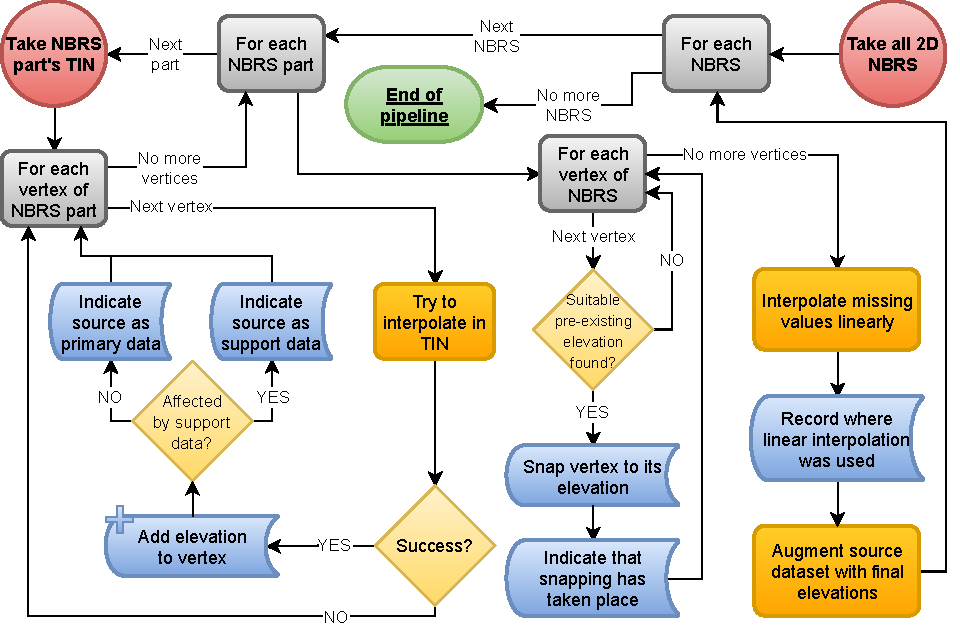
\includegraphics[width=0.9\linewidth]{final_report/figs/elevation_interpolation.pdf}
    \caption{Flowchart-style illustration of the elevation interpolation step of the pipeline.}
    \label{fig:elevationinterpolationflow}
\end{figure}

\subsubsection{Challenges encountered}

As the tasks carried out in this pipeline step are relatively trivial, all challenges encountered were equally simple to solve. The only part of the implementation that proved to be less straightforward was the tracking of the origin of vertices through the TIN-based interpolation - this required some minor modifications to previous steps. The implemented approach is based on hashing: all DTB points that make it into the subcloud of an NBRS part are stored in a hashed structure at one decimal precision of their coordinates, making it quick to identify whether one of the triangle's vertices are among them, that is being used for the interpolation of an NWB vertex.

\section{Accuracy assessment}
\label{sec:m_accuracyassessment}

As I explained in Section \ref{sub:accuracyoverview} above, the estimation of output accuracy assumes no other influences than that which can be propagated through the interpolation technique relative to the input accuracy, in zones that are properly sampled. The task of identifying such regions and computing output accuracy represent the two main tasks in this step, the details of which are explained in this section.

\subsection{Detecting regions with poor sampling}
\label{sub:m_accuracypoorsampling}

\subsubsection{Details of sampling-related assumption}

The circumstance that local sampling density \textit{below a threshold value} does not affect interpolation accuracy is proven by previous work in this field, as mentioned in my literature review results. Of particular importance for us is \cite{guo_etal_2010}, which provides the most amount of detail on this topic. Neither this work, nor any other work to my knowledge derives an explicit mathematical formula that expresses a relationship between local sampling density and output accuracy below the threshold level, but this is not strictly necessary for my research, for a specific reason.

AHN3 has a nominal mean point posting distance of around 30 to 40 centimetres, which I found to be even lower in practice, especially in flat areas such as road surfaces. Considering that the dataset has a vertical and horizontal accuracy of around 15 to 20 centimetres at two standard deviations, we may start to suspect that the surface is heavily oversampled. This happens to an extent, where in practice, a noticeable amount of small-scale elevation scatter becomes observable in the output TIN surfaces. This is due to Lidar \textit{noise}, rather than systematic errors due to local variations in sampling density - no \textit{meaningful} elevation variation is expected on such a small scale.

At such exceptionally dense baseline sampling rates, typical small-scale variations in local sampling density are of no consequence regarding the overall output accuracy. This is simply because these variations will not bring down the local point density to anywhere near to the threshold below which output accuracy would start do deteriorate. 

\subsubsection{Picking an appropriate threshold}

The thresholds I used are based on the results of \cite{guo_etal_2010}. They concluded that in the case of general terrain (not roads specifically) modelled by a raster DTM at a 0.5 m resolution, RMSE with respect to control points does not significantly decrease below 0.2 points per grid cell. In other words, 0.2 points per 0.25 m\textsuperscript{2} appears to be sufficient, or equivalently, 0.8 points per 1 m\textsuperscript{2}. This is in sharp contrast with AHN3's density of 6 to 10 points per 1 m\textsuperscript{2}, especially if we consider that we are only interested in flat surfaces, whereas the results in \cite{guo_etal_2010} are based on areas with a considerable amount of surface ruggedness and used Lidar data with inferior accuracy compared to AHN3.

The extra points may be useful for detecting small-scale features (such as e.g. small slumps in the roads surface), as well as better characterising the edges of roads. However, if we look at the problem strictly from the point of view of the 3D conversion of NWB, then we are only interested in monitoring where the point density goes below the threshold, above which the RMSE with respect to surveyed control points remains relatively constant. If we assume that about 1 point per 1 m\textsuperscript{2} is sufficient to characterise a rugged surface using Lidar, then we could consider drops of up to 90\% in AHN3's point density to be acceptable.

To make sure I use a conservative value, I opted to stay somewhat above the threshold that follows from the above thought process. At each NWB vertex, I examine the number of TIN vertices that fall within 3 metres of it, and if it is less than 3 points, then flag the output accuracy at that point to be unreliable. This corresponds to a a threshold of 3 points per 1 m\textsuperscript{2}. Notably, this threshold deems it reasonable to regard most elevations reliable, which were interpolated inside (wholly or partially) medium-sized gaps resulting from vehicles or other stationary objects on the roads, as well as some that are found in regions where only DTB coverage is available.

\subsubsection{Types of areas violating the assumption}

The local sampling density must drop by more than 60-70\% to reach the above minimum threshold. This means that it only happens in extreme events, such as e.g. occlusion with no DTB coverage. As we lack a mathematical formulation describing the exact nature of the influence below the threshold sampling rate, the best we can do is mark the accuracy of vertices falling into such areas as \textit{"unknown"} in the output.

The first type of area with such poor sampling is the type with no, or almost no Lidar coverage. These areas correspond to centreline vertices which were either excluded from the TIN construction process (by not being included in an NBRS part due to a lack of measurements locally), and ones which \textit{are} in NBRS parts, but do not fall on the TIN-modelled road surface in 2D (most commonly, due to incorrect georeferencing). Both types are given elevation values based on fitting a polynomial model just after interpolating in the underlying TIN. These points are therefore already identified by this circumstance, and need no additional processing.

The second type of area with poor sampling is characterised by an insufficient amount of detail in the TIN. My argumentation in Section \ref{sub:accuracyoverview} specifies that I evaluate this on the basis on checking how big the areas of triangles are, and how long their circumference is, and comparing this with the scale of the input's standard error. While it appears beneficial at a first glance to sample the road surfaces as densely as possible, this is not the case in practice. As I mentioned in Section \ref{sec:lidaraccuracy}, previous research indicated that sampling flat surfaces at typical Lidar posting distances corresponds to oversampling the mathematical surface they can be represented by.

\subsection{Effect of interpolation of accuracy}
\label{sub:m_accuracyinterpolation}

Theoretical proof suggests that the interpolation step generally increases, rather than deteriorates the output accuracy. This can intuitively be thought of as being the result of basing each output elevation on the combined information stored in the three vertices of the triangle in which the location of found, where the value is being interpolated.

This is contrary to what one might assume based on thinking about the pipeline as a whole, but both in practice and in theory, it is the \textit{other} influences on accuracy that generally have the opposite effect. For instance, problems with ground filtering and a sparse local sampling may result in a drop in accuracy locally. However, the interpolation itself has no such effect on the output under normal circumstances. We can thus assert that the formal accuracy of the output will \textit{mostly} increase relative to the input in regions where the local local sampling density does not fall below the threshold of 3 points per 1 m\textsuperscript{2}. I write \textit{mostly}, because there is one exception to this rule: in triangles that are very steep, the combined effects of vertical and horizontal error in the input may entail a significant \textit{increase} in the vertical error, which I will assess numerically after introducing the error propagation formula below (as derived in \cite{fan_etal_2014}).

Let $\sigma_{z_{vx}}^{2}$ denote the elevation variance of the vertices of the triangle, and $\sigma_{xy_{vx}}^{2}$ denote the horizontal variance. Since AHN3 has no vertex-level accuracy specified, we may assume that all vertices, of all triangles take this value. I make the conservative assumption that the better accuracy of DTB relative to AHN3 only holds if all three vertices of a triangle are from DTB - otherwise, DTB vertices also use AHN3's accuracy. We may then express the relationship between the elevation accuracy at the point of interpolation $\sigma_{z_{pt}}^{2}$ as

$\sigma_{z_{pt}}^{2} = M\left(\sigma_{z_{vx}}^{2} + \sigma_{z_{node}}^{2}\left(tan\left(\alpha_x\right)^2 + tan\left(\alpha_y\right)^2\right)\right)$

where $tan\left(\alpha_x\right)^2$ and $tan\left(\alpha_y\right)^2$ correspond to the angle between the triangle's plane and the X and Y axes of the CRS. The expression takes into account the steepness of the plane to be able to propagate the horizontal error, hence the necessity of computing these angles. The variable $M$ is a parameter that needs to be pre-computed for each triangle, as it depends on their 3D geometry. The underlying sizeable formula will not be listed here as it is not relevant to this discussion, please refer to the original paper for it.

The expression is, in essence, a sum of the input variances scaled by geometric variables. Most importantly $M$ has a range between about 1/3 and 1, taking its lowest value around the centroid of the triangle, and increasing to 1 at the triangle's vertices. Intuitively, the closer we are interpolating to one of the vertices, the smaller the other two vertices' influence is going to be due to the nature of TIN-linear interpolation. We are thereby gradually taking into account less and less information, decreasing to the minimum at the vertices, where only one input elevation measurement is considered.

Substituting values into the above formula with $M=0.5$ reveals that applying TIN-linear interpolation to nearly horizontal surfaces will yield on average about 50\% lower elevation variances than the range into which the input variances fall. For instance, a triangle with a 2-degree inclination and a 10-centimetre vertical and horizontal variance (similar to AHN3) yields an output elevation variance of 5 cm, or equivalently, a 10 cm vertical accuracy at two standard deviations (to make it easier to compare with AHN3's accuracy, which is also specified in terms of two standard deviations). Increasing the inclination to 45 degrees decreases the vertical accuracy of the interpolation to 30 cm, which is worse than that of the input.

Such steep roads are rare in reality, and practically absent in The Netherlands - for Dutch roads, the accuracy is still expected to increase, not decrease. However, oversampling the surfaces too heavily with a non-zero stochastic scatter in the elevations can yield small artefact triangles that are inclined anomalously. These inclinations are meaningless, as they do not represent the overall (or local) geometry of the underlying road surfaces, and care should thus be exercised when interpreting the accuracy assessment values of results that were generated using most of the original Lidar points. More information on this topic is found in Section \ref{sec:accuracy}.

\subsection{Evaluating TIN surface completeness}
\label{sub:m_accuracycompleteness}

To evaluate how complete the generated TIN road surfaces are relative to the true road surfaces, I relied on a visual comparison of the TINs with the subclouds, as well as on an external dataset called BGT. Like AHN3 and DTB, it is a Dutch open data geospatial dataset and it is maintained by Kadaster, the national cadastral agency. It is a topographical map of the country which contains a wide range of classified areal features - such as building extents, city extents, and \textit{road} extents.

Like NWB, BGT is also primarily intended to offer good topological accuracy, thus its 2D georeferencing is also relatively crude. However, upon a comparison with satellite imagery, I deemed its road polygons reliable and accurate enough to serve as a reference against which my results can be compared. To make the comparison, I plotted some of the TINs my implementation against the relevant BGT road outlines in 2D and assessed the agreement between them visually. The results of this step, as well as a comparison of BGT and NWB with satellite imagery, is shown in Figure \ref{fig:bgtcomparison}.

\section{Comparison with commercial results}
\label{sec:m_comparison}

From the previous section, we know that the academic results have an output standard elevation error that is either on par with that of the input, or better - with the exception of areas detected as having been too poorly sampled to be given an output accuracy value this way. A simple method to evaluate the overall quality and accuracy of the commercial results is made possible by this. Examining variations in the disagreement between the elevations predicted by the academic and commercial results reveals where the commercial results significantly violate the range of possible values that are set by the academic results and their local standard errors. In other words, where the academic elevation estimates have associated standard error values, we can use them as a reference, against which the commercial results can be benchmarked, both visually (on comparison plots) and quantitatively.

In regions where the academic results are uncertain, the commercial results are in most cases also necessarily uncertain, because the same datasets were used in their production. In such places, the comparison relies on human interpretation. Places where the accuracy estimate is missing due to local problems with growing the TIN surface represent rare exceptions to this rule. In such places, the true size of the road may be larger than it appears in the model. In these rare cases it is possible that the commercial results used support locally that the academic results did not; one such scenario will be presented in the next chapter.

In all areas, computing and plotting the residuals between the two sets of results yields further insight into trends in the differences. Correlating these with the comparison plots of the elevation series, as well as 3D plots of the data and underlying AHN3 and DTB points, aids the human interpretation of the differences. Generating Root Mean Squared Error (RMSE) values on the level of wegvakken, as well as cumulatively for entire testing datasets, is also a method I employed. The RMSE is given by

$\sqrt{\frac{\sum_{t=1}^{T}\left(z_{a,t} - z_{c,t}\right)^2}{T}}$

where are samples in a profile are from $t=1$ to $T$, and where $z_{c,t}$ denotes the elevation estimated by my method, and $z_{c,t}$ denotes the commercial result at the same location.

I perform the comparison on individual wegvakken. The distances from the first vertex of the wegvak along the profile from $t=1$ to $T$ are computed, this is what the elevation series are plotted against. The residuals (and thus, the RMSE values) are based on values taken by $z_{a,t_{nwb}} - z_{c,t_{nwb}}$ where $t_{nwb}$ corresponds to original NWB vertices. Both the academic and the commercial pipelines use vertex densification, but the resulting vertices are not located in the same place. Thus, the residuals and the RMSE values describe only how well the two methods agree at the \textit{original} NWB vertices.

\section{Programming framework}
\label{sec:programming}

The implementation part of this project is intended to investigate how well each step of the pipeline works in practice, how well they work together as a pipeline, and how accurate their output is. In turn, these serve the purpose of answering the research questions detailed in Section [REF]. In addition, implementation-related tasks were also important in iteratively revising the methods based on the practical experience gained in the process, making them better adapted to real-life scenarios (and as result, more relevant to reusers).

\subsubsection{Notes on performance}

As the implementation is intended for demonstration and reference purposes, it is by no means ready for all types of academic and commercial use out of the box. One limiting factor in this sense is the lack of a scaling mechanism in the implementation, as such considerations were not part of this research. Furthermore, I developed all parts of the pipeline in Python 3.8, which means that the code is more concise than a binary implementation would be, but its performance is worse. To improve performance, I relied on binary-based libraries such as numpy, and parts of scipy wherever they could help decrease runtimes. I also always paid attention to avoid increasing computational complexity unnecessarily. In addition, I also used hashing (Python dictionaries and sets) extensively, which are also known to benefit performance greatly. Many of these uses of hashing are mentioned previous sections explicitly, and wherever I mention using KD-trees, I refer to building code on top of the binary implementation in scipy. Uses of numpy are so pervasive in the code, that I opted not to mention them explicitly in the text.

While geometries (and geometry operations) are often handled in shapely, I avoided its use in all cases where geometries are bulk-processed via long iterations. I found that implementing the geometry operations from first principles in numpy in such cases resulted in a noticeable gain in performance in such scenarios.

Unfortunately, the implementation of active contour optimisation in scikit-image is mostly based on native Python iterations, not on a binary package. This circumstance, in conjunction with the large number of vector inner products that the attractor map generation requires, means that the computational complexity of the active contour-related part of my software is a magnitude slower than all other parts.

\subsubsection{GitHub release and code structure}

I released the source code of the implementation in the following GitHub repository:
\url{https://github.com/kriskenesei/geo2020-modules}. Most functionality resides in the class \codeword{nbrs_manager} inside the file \codeword{nbrs_generation.py}. I factored out some functionality into \codeword{lib_shared.py} to somewhat simplify the code in \codeword{nbrs_generation.py}. Both files contain an extensive set of docstrings, as well as inline guidance on what each part of the code does. The intended audience of this information includes those simply interested in knowing more about the practical aspects of processing that underlies this research, as well as potential reusers.

The class \codeword{nbrs_manager} holds a range of intermediate results, as well as final results in class variables. The class is intended to be instantiated with the road network NWB, followed by the invocation of class methods corresponding to each pipeline step. In addition, vertex densification is also implemented as its own class method, and a range of smaller methods are provided for basic operations such as setting individual wegvak geometry, as well as writing the intermediate results of each pipeline step to disk separately. The arguments of the methods generally take input file paths and/or parameters (for processing steps) and  output file paths and/or parameters (for output writing operations). The structure of the first part of the next chapter is modelled on the steps one would take to run my software with NWB, AHN3 and DTB, to create a stronger link between the explanations and the code itself. These explanations of how the software was used to generate the results will be illustrated with example calls, but a condensed explanation can also be found in the docstring of \codeword{nbrs_manager} of the necessary calls, and a set of example calls are also provided at the end of the file \codeword{nbrs_generation.py}.